\documentclass[twoside]{book}

% Packages required by doxygen
\usepackage{fixltx2e}
\usepackage{calc}
\usepackage{doxygen}
\usepackage[export]{adjustbox} % also loads graphicx
\usepackage{graphicx}
\usepackage[utf8]{inputenc}
\usepackage{makeidx}
\usepackage{multicol}
\usepackage{multirow}
\PassOptionsToPackage{warn}{textcomp}
\usepackage{textcomp}
\usepackage[nointegrals]{wasysym}
\usepackage[table]{xcolor}

% Font selection
\usepackage[T1]{fontenc}
\usepackage[scaled=.90]{helvet}
\usepackage{courier}
\usepackage{amssymb}
\usepackage{sectsty}
\renewcommand{\familydefault}{\sfdefault}
\allsectionsfont{%
  \fontseries{bc}\selectfont%
  \color{darkgray}%
}
\renewcommand{\DoxyLabelFont}{%
  \fontseries{bc}\selectfont%
  \color{darkgray}%
}
\newcommand{\+}{\discretionary{\mbox{\scriptsize$\hookleftarrow$}}{}{}}

% Page & text layout
\usepackage{geometry}
\geometry{%
  a4paper,%
  top=2.5cm,%
  bottom=2.5cm,%
  left=2.5cm,%
  right=2.5cm%
}
\tolerance=750
\hfuzz=15pt
\hbadness=750
\setlength{\emergencystretch}{15pt}
\setlength{\parindent}{0cm}
\setlength{\parskip}{3ex plus 2ex minus 2ex}
\makeatletter
\renewcommand{\paragraph}{%
  \@startsection{paragraph}{4}{0ex}{-1.0ex}{1.0ex}{%
    \normalfont\normalsize\bfseries\SS@parafont%
  }%
}
\renewcommand{\subparagraph}{%
  \@startsection{subparagraph}{5}{0ex}{-1.0ex}{1.0ex}{%
    \normalfont\normalsize\bfseries\SS@subparafont%
  }%
}
\makeatother

% Headers & footers
\usepackage{fancyhdr}
\pagestyle{fancyplain}
\fancyhead[LE]{\fancyplain{}{\bfseries\thepage}}
\fancyhead[CE]{\fancyplain{}{}}
\fancyhead[RE]{\fancyplain{}{\bfseries\leftmark}}
\fancyhead[LO]{\fancyplain{}{\bfseries\rightmark}}
\fancyhead[CO]{\fancyplain{}{}}
\fancyhead[RO]{\fancyplain{}{\bfseries\thepage}}
\fancyfoot[LE]{\fancyplain{}{}}
\fancyfoot[CE]{\fancyplain{}{}}
\fancyfoot[RE]{\fancyplain{}{\bfseries\scriptsize Generated by Doxygen }}
\fancyfoot[LO]{\fancyplain{}{\bfseries\scriptsize Generated by Doxygen }}
\fancyfoot[CO]{\fancyplain{}{}}
\fancyfoot[RO]{\fancyplain{}{}}
\renewcommand{\footrulewidth}{0.4pt}
\renewcommand{\chaptermark}[1]{%
  \markboth{#1}{}%
}
\renewcommand{\sectionmark}[1]{%
  \markright{\thesection\ #1}%
}

% Indices & bibliography
\usepackage{natbib}
\usepackage[titles]{tocloft}
\setcounter{tocdepth}{3}
\setcounter{secnumdepth}{5}
\makeindex

% Hyperlinks (required, but should be loaded last)
\usepackage{ifpdf}
\ifpdf
  \usepackage[pdftex,pagebackref=true]{hyperref}
\else
  \usepackage[ps2pdf,pagebackref=true]{hyperref}
\fi
\hypersetup{%
  colorlinks=true,%
  linkcolor=blue,%
  citecolor=blue,%
  unicode%
}

% Custom commands
\newcommand{\clearemptydoublepage}{%
  \newpage{\pagestyle{empty}\cleardoublepage}%
}

\usepackage{caption}
\captionsetup{labelsep=space,justification=centering,font={bf},singlelinecheck=off,skip=4pt,position=top}

%===== C O N T E N T S =====

\begin{document}

% Titlepage & ToC
\hypersetup{pageanchor=false,
             bookmarksnumbered=true,
             pdfencoding=unicode
            }
\pagenumbering{alph}
\begin{titlepage}
\vspace*{7cm}
\begin{center}%
{\Large Bandit\+P\+AM }\\
\vspace*{1cm}
{\large Generated by Doxygen 1.8.13}\\
\end{center}
\end{titlepage}
\clearemptydoublepage
\pagenumbering{roman}
\tableofcontents
\clearemptydoublepage
\pagenumbering{arabic}
\hypersetup{pageanchor=true}

%--- Begin generated contents ---
\chapter{Bandit\+P\+AM\+: Almost Linear-\/\+Time $\ast$k$\ast$-\/\+Medoids Clustering}
\label{index}\hypertarget{index}{}\input{index}
\chapter{Hierarchical Index}
\section{Class Hierarchy}
This inheritance list is sorted roughly, but not completely, alphabetically\+:\begin{DoxyCompactList}
\item \contentsline{section}{K\+Medoids}{\pageref{classKMedoids}}{}
\begin{DoxyCompactList}
\item \contentsline{section}{K\+Medoids\+Wrapper}{\pageref{classKMedoidsWrapper}}{}
\end{DoxyCompactList}
\item \contentsline{section}{Log\+Helper}{\pageref{structLogHelper}}{}
\end{DoxyCompactList}

\chapter{Class Index}
\section{Class List}
Here are the classes, structs, unions and interfaces with brief descriptions\+:\begin{DoxyCompactList}
\item\contentsline{section}{\hyperlink{classKMedoids}{K\+Medoids} \\*Class implementation for running \hyperlink{classKMedoids}{K\+Medoids} methods }{\pageref{classKMedoids}}{}
\item\contentsline{section}{\hyperlink{classKMedoidsWrapper}{K\+Medoids\+Wrapper} \\*Python wrapper for \hyperlink{classKMedoids}{K\+Medoids} class }{\pageref{classKMedoidsWrapper}}{}
\item\contentsline{section}{\hyperlink{structLogHelper}{Log\+Helper} \\*Logging class for structured \hyperlink{classKMedoids}{K\+Medoids} logs }{\pageref{structLogHelper}}{}
\end{DoxyCompactList}

\chapter{File Index}
\section{File List}
Here is a list of all documented files with brief descriptions\+:\begin{DoxyCompactList}
\item\contentsline{section}{/home/esfrankel/\+Desktop/\+Bandit\+P\+A\+M/headers/{\bfseries kmedoids\+\_\+ucb.\+hpp} }{\pageref{kmedoids__ucb_8hpp}}{}
\item\contentsline{section}{/home/esfrankel/\+Desktop/\+Bandit\+P\+A\+M/src/\hyperlink{kmedoids__ucb_8cpp}{kmedoids\+\_\+ucb.\+cpp} }{\pageref{kmedoids__ucb_8cpp}}{}
\item\contentsline{section}{/home/esfrankel/\+Desktop/\+Bandit\+P\+A\+M/src/\hyperlink{kmedoids__pywrapper_8cpp}{kmedoids\+\_\+pywrapper.\+cpp} }{\pageref{kmedoids__pywrapper_8cpp}}{}
\item\contentsline{section}{/home/esfrankel/\+Desktop/\+Bandit\+P\+A\+M/src/\hyperlink{main_8cpp}{main.\+cpp} }{\pageref{main_8cpp}}{}
\end{DoxyCompactList}

\chapter{Class Documentation}
\hypertarget{classKMedoids}{}\doxysection{KMedoids Class Reference}
\label{classKMedoids}\index{KMedoids@{KMedoids}}


Class implementation for running \mbox{\hyperlink{classKMedoids}{KMedoids}} methods.  




{\ttfamily \#include $<$kmedoids\+\_\+ucb.\+hpp$>$}



Inheritance diagram for KMedoids\+:
\nopagebreak
\begin{figure}[H]
\begin{center}
\leavevmode
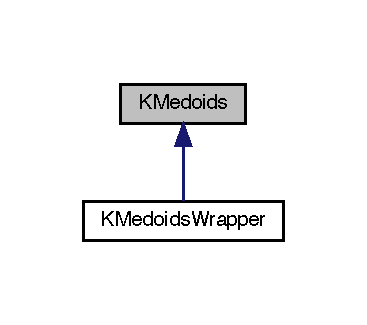
\includegraphics[width=176pt]{classKMedoids__inherit__graph}
\end{center}
\end{figure}
\doxysubsection*{Public Member Functions}
\begin{DoxyCompactItemize}
\item 
\mbox{\hyperlink{classKMedoids_aa94dfc65454f847af5d08a2d7b816bb4}{KMedoids}} (int \mbox{\hyperlink{classKMedoids_a3365e728fd524c0be2fbab0b58e3a4cd}{n\+\_\+medoids}}=5, std\+::string \mbox{\hyperlink{classKMedoids_a849662ecdbd5164ab37f4bd4f3223344}{algorithm}}=\char`\"{}Bandit\+PAM\char`\"{}, int \mbox{\hyperlink{classKMedoids_a8d319c1a783be7c06205bf855b4976b5}{verbosity}}=0, int \mbox{\hyperlink{classKMedoids_a3f8f9d261e721749f14f30dacfe9aa03}{max\+\_\+iter}}=1000, std\+::string \mbox{\hyperlink{classKMedoids_a3cf57e612442072fb377b1714fc5e12e}{log\+Filename}}=\char`\"{}KMedoids\+Logfile\char`\"{})
\begin{DoxyCompactList}\small\item\em Class implementation for running \mbox{\hyperlink{classKMedoids}{KMedoids}} methods. \end{DoxyCompactList}\item 
\mbox{\hyperlink{classKMedoids_a82710100b6fb5820c10bc3f796ed62ff}{$\sim$\+KMedoids}} ()
\begin{DoxyCompactList}\small\item\em Destroys \mbox{\hyperlink{classKMedoids}{KMedoids}} object. \end{DoxyCompactList}\item 
void \mbox{\hyperlink{classKMedoids_ae241800e72a6b4a677333ffbf06e1798}{fit}} (arma\+::mat input\+Data, std\+::string loss)
\begin{DoxyCompactList}\small\item\em Finds medoids for the input data under identified loss function. \end{DoxyCompactList}\item 
arma\+::rowvec \mbox{\hyperlink{classKMedoids_a26aa9827d2541626d959dc984f0f9bcb}{get\+Medoids\+Final}} ()
\begin{DoxyCompactList}\small\item\em Returns the final medoids. \end{DoxyCompactList}\item 
arma\+::rowvec \mbox{\hyperlink{classKMedoids_a54370d8d0f5c500f5deb859a9eab891c}{get\+Medoids\+Build}} ()
\begin{DoxyCompactList}\small\item\em Returns the build medoids. \end{DoxyCompactList}\item 
arma\+::rowvec \mbox{\hyperlink{classKMedoids_a89474787892880381e4d0282de541d03}{get\+Labels}} ()
\begin{DoxyCompactList}\small\item\em Returns the medoid assignments for each datapoint. \end{DoxyCompactList}\item 
int \mbox{\hyperlink{classKMedoids_a2c8d55468ebe909229ea7bcdb50e8351}{get\+Steps}} ()
\begin{DoxyCompactList}\small\item\em Returns the number of swap steps. \end{DoxyCompactList}\item 
int \mbox{\hyperlink{classKMedoids_ad738dc6b5a2dafa1ff4aeab807d6407d}{get\+NMedoids}} ()
\begin{DoxyCompactList}\small\item\em Returns the number of medoids. \end{DoxyCompactList}\item 
void \mbox{\hyperlink{classKMedoids_ad28860f50c0b5a4968f99d103b3de06f}{set\+NMedoids}} (int new\+\_\+num)
\begin{DoxyCompactList}\small\item\em Sets the number of medoids. \end{DoxyCompactList}\item 
std\+::string \mbox{\hyperlink{classKMedoids_a01a1bf63fdd2cd8b389c3f1c0619388f}{get\+Algorithm}} ()
\begin{DoxyCompactList}\small\item\em Returns the algorithm for \mbox{\hyperlink{classKMedoids}{KMedoids}}. \end{DoxyCompactList}\item 
void \mbox{\hyperlink{classKMedoids_a1a6dbc45f5d83bded48bf86cbc2690ad}{set\+Algorithm}} (std\+::string new\+\_\+alg)
\begin{DoxyCompactList}\small\item\em Sets the algorithm for \mbox{\hyperlink{classKMedoids}{KMedoids}}. \end{DoxyCompactList}\item 
int \mbox{\hyperlink{classKMedoids_a8d5372adbed828602f9311dbe9c70198}{get\+Verbosity}} ()
\begin{DoxyCompactList}\small\item\em Returns the verbosity for \mbox{\hyperlink{classKMedoids}{KMedoids}}. \end{DoxyCompactList}\item 
void \mbox{\hyperlink{classKMedoids_a8d03726bbd66ffc6d2c202d2a3cf40d5}{set\+Verbosity}} (int new\+\_\+ver)
\begin{DoxyCompactList}\small\item\em Sets the verbosity for \mbox{\hyperlink{classKMedoids}{KMedoids}}. \end{DoxyCompactList}\item 
int \mbox{\hyperlink{classKMedoids_ac0569206113015abb38954f78a194eb5}{get\+Max\+Iter}} ()
\begin{DoxyCompactList}\small\item\em Returns the maximum number of iterations for \mbox{\hyperlink{classKMedoids}{KMedoids}}. \end{DoxyCompactList}\item 
void \mbox{\hyperlink{classKMedoids_ae1a84d5509090d31cd1c04616fd615f3}{set\+Max\+Iter}} (int new\+\_\+max)
\begin{DoxyCompactList}\small\item\em Sets the maximum number of iterations for \mbox{\hyperlink{classKMedoids}{KMedoids}}. \end{DoxyCompactList}\item 
std\+::string \mbox{\hyperlink{classKMedoids_ad5982ef2a71cce9f1f45b98c55350391}{get\+Logfile\+Name}} ()
\begin{DoxyCompactList}\small\item\em Returns the log filename for \mbox{\hyperlink{classKMedoids}{KMedoids}}. \end{DoxyCompactList}\item 
void \mbox{\hyperlink{classKMedoids_a45f89770245bff638e25bcd39ab52013}{set\+Log\+Filename}} (std\+::string new\+\_\+lname)
\begin{DoxyCompactList}\small\item\em Sets the log filename for \mbox{\hyperlink{classKMedoids}{KMedoids}}. \end{DoxyCompactList}\item 
void \mbox{\hyperlink{classKMedoids_ab442bf7198be7a48a7eb5901ac7ca571}{set\+Loss\+Fn}} (std\+::string loss)
\begin{DoxyCompactList}\small\item\em Sets the loss function. \end{DoxyCompactList}\end{DoxyCompactItemize}
\doxysubsection*{Private Member Functions}
\begin{DoxyCompactItemize}
\item 
void \mbox{\hyperlink{classKMedoids_afb08301b64e5be0b9f274a14908c7869}{fit\+\_\+bpam}} (arma\+::mat input\+Data)
\begin{DoxyCompactList}\small\item\em Runs Bandit\+PAM algorithm. \end{DoxyCompactList}\item 
void \mbox{\hyperlink{classKMedoids_a79fbb790f9f31bcaf1daa05e5eb5daa8}{fit\+\_\+naive}} (arma\+::mat input\+Data)
\begin{DoxyCompactList}\small\item\em Runs naive PAM algorithm. \end{DoxyCompactList}\item 
void \mbox{\hyperlink{classKMedoids_accedac4456cc27abbfd1a9ab1a0a5526}{build\+\_\+naive}} (arma\+::mat \&\mbox{\hyperlink{classKMedoids_afca7201861fc3c605ba25e059cd58764}{data}}, arma\+::rowvec \&medoid\+Indices)
\begin{DoxyCompactList}\small\item\em Build step for the naive algorithm. \end{DoxyCompactList}\item 
void \mbox{\hyperlink{classKMedoids_a08035b01998e5365dcfb3638dcf8ed53}{swap\+\_\+naive}} (arma\+::mat \&\mbox{\hyperlink{classKMedoids_afca7201861fc3c605ba25e059cd58764}{data}}, arma\+::rowvec \&medoid\+Indices)
\begin{DoxyCompactList}\small\item\em Swap step for the naive algorithm. \end{DoxyCompactList}\item 
void \mbox{\hyperlink{classKMedoids_af650596c4cf9746564f2ea3dce3e113d}{build}} (arma\+::mat \&\mbox{\hyperlink{classKMedoids_afca7201861fc3c605ba25e059cd58764}{data}}, arma\+::rowvec \&medoid\+Indices, arma\+::mat \&medoids)
\begin{DoxyCompactList}\small\item\em Build step for Bandit\+PAM. \end{DoxyCompactList}\item 
void \mbox{\hyperlink{classKMedoids_a320b25fdc5b8f66a81ea6d3b9a0c105c}{build\+\_\+sigma}} (arma\+::mat \&\mbox{\hyperlink{classKMedoids_afca7201861fc3c605ba25e059cd58764}{data}}, arma\+::rowvec \&best\+\_\+distances, arma\+::rowvec \&sigma, arma\+::uword batch\+\_\+size, bool use\+\_\+absolute)
\begin{DoxyCompactList}\small\item\em Calculates confidence intervals in build step. \end{DoxyCompactList}\item 
arma\+::rowvec \mbox{\hyperlink{classKMedoids_a1ba213f14eb7577414b9bc6c445fcb2a}{build\+\_\+target}} (arma\+::mat \&\mbox{\hyperlink{classKMedoids_afca7201861fc3c605ba25e059cd58764}{data}}, arma\+::uvec \&target, size\+\_\+t batch\+\_\+size, arma\+::rowvec \&best\+\_\+distances, bool use\+\_\+absolute)
\begin{DoxyCompactList}\small\item\em Estimates the mean reward for each arm in build step. \end{DoxyCompactList}\item 
void \mbox{\hyperlink{classKMedoids_a3d49e6e8d2b6dbcc1d357b9ee3dfdfb4}{swap}} (arma\+::mat \&\mbox{\hyperlink{classKMedoids_afca7201861fc3c605ba25e059cd58764}{data}}, arma\+::rowvec \&medoid\+Indices, arma\+::mat \&medoids, arma\+::rowvec \&assignments)
\begin{DoxyCompactList}\small\item\em Swap step for Bandit\+PAM. \end{DoxyCompactList}\item 
void \mbox{\hyperlink{classKMedoids_a83f8605eb570f345553d75ff8674f137}{calc\+\_\+best\+\_\+distances\+\_\+swap}} (arma\+::mat \&\mbox{\hyperlink{classKMedoids_afca7201861fc3c605ba25e059cd58764}{data}}, arma\+::rowvec \&medoid\+Indices, arma\+::rowvec \&best\+\_\+distances, arma\+::rowvec \&second\+\_\+distances, arma\+::rowvec \&assignments)
\begin{DoxyCompactList}\small\item\em Calculates distances in swap step. \end{DoxyCompactList}\item 
arma\+::vec \mbox{\hyperlink{classKMedoids_ab0cece04337d5ca9cfa8637a7f465507}{swap\+\_\+target}} (arma\+::mat \&\mbox{\hyperlink{classKMedoids_afca7201861fc3c605ba25e059cd58764}{data}}, arma\+::rowvec \&medoid\+Indices, arma\+::uvec \&targets, size\+\_\+t batch\+\_\+size, arma\+::rowvec \&best\+\_\+distances, arma\+::rowvec \&second\+\_\+best\+\_\+distances, arma\+::rowvec \&assignments)
\begin{DoxyCompactList}\small\item\em Estimates the mean reward for each arm in swap step. \end{DoxyCompactList}\item 
void \mbox{\hyperlink{classKMedoids_a296c3f0cacab45b5c642516c91979a8c}{swap\+\_\+sigma}} (arma\+::mat \&\mbox{\hyperlink{classKMedoids_afca7201861fc3c605ba25e059cd58764}{data}}, arma\+::mat \&sigma, size\+\_\+t batch\+\_\+size, arma\+::rowvec \&best\+\_\+distances, arma\+::rowvec \&second\+\_\+best\+\_\+distances, arma\+::rowvec \&assignments)
\begin{DoxyCompactList}\small\item\em Calculates confidence intervals in swap step. \end{DoxyCompactList}\item 
double \mbox{\hyperlink{classKMedoids_a4cf0d9c4ecebc5a4bd20a9441dbda711}{calc\+\_\+loss}} (arma\+::mat \&\mbox{\hyperlink{classKMedoids_afca7201861fc3c605ba25e059cd58764}{data}}, arma\+::rowvec \&medoid\+Indices)
\begin{DoxyCompactList}\small\item\em Calculate loss for medoids. \end{DoxyCompactList}\item 
double \mbox{\hyperlink{classKMedoids_a05c9fccee6a00b5ad58bc5a16c9f0cb6}{LP}} (arma\+::mat \&\mbox{\hyperlink{classKMedoids_afca7201861fc3c605ba25e059cd58764}{data}}, int i, int j) const
\begin{DoxyCompactList}\small\item\em LP loss. \end{DoxyCompactList}\item 
double \mbox{\hyperlink{classKMedoids_a6d63f7f2301e6e7b6ecfa892433cec71}{LINF}} (arma\+::mat \&\mbox{\hyperlink{classKMedoids_afca7201861fc3c605ba25e059cd58764}{data}}, int i, int j) const
\begin{DoxyCompactList}\small\item\em L\+\_\+\+INFINITY loss. \end{DoxyCompactList}\item 
double \mbox{\hyperlink{classKMedoids_a56028b6ad37c2064aab129bcbf475816}{cos}} (arma\+::mat \&\mbox{\hyperlink{classKMedoids_afca7201861fc3c605ba25e059cd58764}{data}}, int i, int j) const
\begin{DoxyCompactList}\small\item\em L2 loss. \end{DoxyCompactList}\item 
double \mbox{\hyperlink{classKMedoids_ad59fdea6100cb2326510cd6352bcd322}{manhattan}} (arma\+::mat \&\mbox{\hyperlink{classKMedoids_afca7201861fc3c605ba25e059cd58764}{data}}, int i, int j) const
\begin{DoxyCompactList}\small\item\em Manhattan loss. \end{DoxyCompactList}\item 
void \mbox{\hyperlink{classKMedoids_af5b9331755cd049afb05af8ecee3aeb5}{check\+Algorithm}} (std\+::string \mbox{\hyperlink{classKMedoids_a849662ecdbd5164ab37f4bd4f3223344}{algorithm}})
\begin{DoxyCompactList}\small\item\em Checks whether algorithm input is valid. \end{DoxyCompactList}\end{DoxyCompactItemize}
\doxysubsection*{Private Attributes}
\begin{DoxyCompactItemize}
\item 
\mbox{\Hypertarget{classKMedoids_adbaa97bad10ef761570874ef94a4fc2a}\label{classKMedoids_adbaa97bad10ef761570874ef94a4fc2a}} 
int {\bfseries lp}
\item 
\mbox{\Hypertarget{classKMedoids_a849662ecdbd5164ab37f4bd4f3223344}\label{classKMedoids_a849662ecdbd5164ab37f4bd4f3223344}} 
std\+::string {\bfseries algorithm}
\begin{DoxyCompactList}\small\item\em options\+: \char`\"{}naive\char`\"{} and \char`\"{}\+Bandit\+PAM\char`\"{} \end{DoxyCompactList}\item 
\mbox{\Hypertarget{classKMedoids_a3f8f9d261e721749f14f30dacfe9aa03}\label{classKMedoids_a3f8f9d261e721749f14f30dacfe9aa03}} 
int {\bfseries max\+\_\+iter}
\begin{DoxyCompactList}\small\item\em maximum number of iterations during \mbox{\hyperlink{classKMedoids_ae241800e72a6b4a677333ffbf06e1798}{KMedoids\+::fit}} \end{DoxyCompactList}\item 
\mbox{\Hypertarget{classKMedoids_a8d319c1a783be7c06205bf855b4976b5}\label{classKMedoids_a8d319c1a783be7c06205bf855b4976b5}} 
int {\bfseries verbosity}
\begin{DoxyCompactList}\small\item\em determines whether \mbox{\hyperlink{classKMedoids_ae241800e72a6b4a677333ffbf06e1798}{KMedoids\+::fit}} outputs a logfile \end{DoxyCompactList}\item 
\mbox{\Hypertarget{classKMedoids_a3365e728fd524c0be2fbab0b58e3a4cd}\label{classKMedoids_a3365e728fd524c0be2fbab0b58e3a4cd}} 
int {\bfseries n\+\_\+medoids}
\begin{DoxyCompactList}\small\item\em number of medoids identified for a given dataset \end{DoxyCompactList}\item 
\mbox{\Hypertarget{classKMedoids_a3cf57e612442072fb377b1714fc5e12e}\label{classKMedoids_a3cf57e612442072fb377b1714fc5e12e}} 
std\+::string {\bfseries log\+Filename}
\begin{DoxyCompactList}\small\item\em name of the logfile output (verbosity permitting) \end{DoxyCompactList}\item 
\mbox{\Hypertarget{classKMedoids_afca7201861fc3c605ba25e059cd58764}\label{classKMedoids_afca7201861fc3c605ba25e059cd58764}} 
arma\+::mat {\bfseries data}
\begin{DoxyCompactList}\small\item\em input data used during \mbox{\hyperlink{classKMedoids_ae241800e72a6b4a677333ffbf06e1798}{KMedoids\+::fit}} \end{DoxyCompactList}\item 
\mbox{\Hypertarget{classKMedoids_a45310cf654a48d10b5ad5727ad4ef642}\label{classKMedoids_a45310cf654a48d10b5ad5727ad4ef642}} 
arma\+::rowvec {\bfseries labels}
\begin{DoxyCompactList}\small\item\em assignments of each datapoint to its medoid \end{DoxyCompactList}\item 
\mbox{\Hypertarget{classKMedoids_a604881068bc30237190db6fc73f2d0c7}\label{classKMedoids_a604881068bc30237190db6fc73f2d0c7}} 
arma\+::rowvec {\bfseries medoid\+\_\+indices\+\_\+build}
\begin{DoxyCompactList}\small\item\em medoids at the end of build step \end{DoxyCompactList}\item 
\mbox{\Hypertarget{classKMedoids_aac1178a6e7f0da5338efb94e49def9dd}\label{classKMedoids_aac1178a6e7f0da5338efb94e49def9dd}} 
arma\+::rowvec {\bfseries medoid\+\_\+indices\+\_\+final}
\begin{DoxyCompactList}\small\item\em medoids at the end of the swap step \end{DoxyCompactList}\item 
\mbox{\Hypertarget{classKMedoids_a048a16c6055667e4a492c83d6ad25cac}\label{classKMedoids_a048a16c6055667e4a492c83d6ad25cac}} 
double(KMedoids\+::$\ast$ {\bfseries loss\+Fn} )(arma\+::mat \&\mbox{\hyperlink{classKMedoids_afca7201861fc3c605ba25e059cd58764}{data}}, int i, int j) const
\begin{DoxyCompactList}\small\item\em loss function used during \mbox{\hyperlink{classKMedoids_ae241800e72a6b4a677333ffbf06e1798}{KMedoids\+::fit}} \end{DoxyCompactList}\item 
\mbox{\Hypertarget{classKMedoids_ac36a9e6347281ff72dc3ccd677f8c45a}\label{classKMedoids_ac36a9e6347281ff72dc3ccd677f8c45a}} 
void(KMedoids\+::$\ast$ {\bfseries fit\+Fn} )(arma\+::mat input\+Data)
\begin{DoxyCompactList}\small\item\em function used for finding medoids (from algorithm) \end{DoxyCompactList}\item 
\mbox{\Hypertarget{classKMedoids_a3c2f6a89220d392c50f4791dd6f5773b}\label{classKMedoids_a3c2f6a89220d392c50f4791dd6f5773b}} 
\mbox{\hyperlink{structLogHelper}{Log\+Helper}} {\bfseries log\+Helper}
\begin{DoxyCompactList}\small\item\em helper object for making formatted logs \end{DoxyCompactList}\item 
\mbox{\Hypertarget{classKMedoids_a48502b4eca5c4eea065659afde6abb53}\label{classKMedoids_a48502b4eca5c4eea065659afde6abb53}} 
int {\bfseries steps}
\begin{DoxyCompactList}\small\item\em number of actual swap iterations taken by the algorithm \end{DoxyCompactList}\item 
\mbox{\Hypertarget{classKMedoids_a8777933aacdc528fc4ac18d47fd3fa29}\label{classKMedoids_a8777933aacdc528fc4ac18d47fd3fa29}} 
const double {\bfseries precision} = 0.\+001
\begin{DoxyCompactList}\small\item\em bound for double comparison precision \end{DoxyCompactList}\item 
\mbox{\Hypertarget{classKMedoids_abe265fbf9b607f20544b9b32e923a893}\label{classKMedoids_abe265fbf9b607f20544b9b32e923a893}} 
const size\+\_\+t {\bfseries batch\+Size} = 100
\begin{DoxyCompactList}\small\item\em batch size for computation steps \end{DoxyCompactList}\end{DoxyCompactItemize}
\doxysubsection*{Static Private Attributes}
\begin{DoxyCompactItemize}
\item 
\mbox{\Hypertarget{classKMedoids_a75a5dc3ec625069a5fc98d133b2c22df}\label{classKMedoids_a75a5dc3ec625069a5fc98d133b2c22df}} 
static const size\+\_\+t {\bfseries build\+Confidence} = 1000
\begin{DoxyCompactList}\small\item\em constant that affects the sensitivity of build confidence bounds \end{DoxyCompactList}\item 
\mbox{\Hypertarget{classKMedoids_aa29c755077f4bae62548cdf608ab0623}\label{classKMedoids_aa29c755077f4bae62548cdf608ab0623}} 
static const size\+\_\+t {\bfseries swap\+Confidence} = 10000
\begin{DoxyCompactList}\small\item\em constant that affects the sensitiviy of swap confidence bounds \end{DoxyCompactList}\end{DoxyCompactItemize}


\doxysubsection{Detailed Description}
Class implementation for running \mbox{\hyperlink{classKMedoids}{KMedoids}} methods. 

\mbox{\hyperlink{classKMedoids}{KMedoids}} class. Creates a \mbox{\hyperlink{classKMedoids}{KMedoids}} object that can be used to find the medoids for a particular set of input data.


\begin{DoxyParams}{Parameters}
{\em n\+Medoids} & Number of medoids/clusters to create \\
\hline
{\em algorithm} & Algorithm used to find medoids; options are \char`\"{}\+Bandit\+PAM\char`\"{} for the \char`\"{}\+Bandit-\/\+PAM\char`\"{} algorithm, or \char`\"{}naive\char`\"{} to use the naive method \\
\hline
{\em verbosity} & Verbosity of the algorithm, 0 will have no log file emitted, 1 will emit a log file \\
\hline
{\em max\+Iter} & The maximum number of iterations the algorithm runs for \\
\hline
{\em log\+Filename} & The name of the output log file \\
\hline
\end{DoxyParams}


\doxysubsection{Constructor \& Destructor Documentation}
\mbox{\Hypertarget{classKMedoids_aa94dfc65454f847af5d08a2d7b816bb4}\label{classKMedoids_aa94dfc65454f847af5d08a2d7b816bb4}} 
\index{KMedoids@{KMedoids}!KMedoids@{KMedoids}}
\index{KMedoids@{KMedoids}!KMedoids@{KMedoids}}
\doxysubsubsection{\texorpdfstring{KMedoids()}{KMedoids()}}
{\footnotesize\ttfamily KMedoids\+::\+KMedoids (\begin{DoxyParamCaption}\item[{int}]{n\+\_\+medoids = {\ttfamily 5},  }\item[{std\+::string}]{algorithm = {\ttfamily \char`\"{}BanditPAM\char`\"{}},  }\item[{int}]{verbosity = {\ttfamily 0},  }\item[{int}]{max\+\_\+iter = {\ttfamily 1000},  }\item[{std\+::string}]{log\+Filename = {\ttfamily \char`\"{}KMedoidsLogfile\char`\"{}} }\end{DoxyParamCaption})}



Class implementation for running \mbox{\hyperlink{classKMedoids}{KMedoids}} methods. 

\mbox{\hyperlink{classKMedoids}{KMedoids}} class. Creates a \mbox{\hyperlink{classKMedoids}{KMedoids}} object that can be used to find the medoids for a particular set of input data.


\begin{DoxyParams}{Parameters}
{\em n\+\_\+medoids} & Number of medoids/clusters to create \\
\hline
{\em algorithm} & Algorithm used to find medoids; options are \char`\"{}\+Bandit\+PAM\char`\"{} for the \char`\"{}\+Bandit-\/\+PAM\char`\"{} algorithm, or \char`\"{}naive\char`\"{} to use the naive method \\
\hline
{\em verbosity} & Verbosity of the algorithm, 0 will have no log file emitted, 1 will emit a log file \\
\hline
{\em max\+\_\+iter} & The maximum number of iterations the algorithm runs for \\
\hline
{\em log\+Filename} & The name of the output log file \\
\hline
\end{DoxyParams}
\mbox{\Hypertarget{classKMedoids_a82710100b6fb5820c10bc3f796ed62ff}\label{classKMedoids_a82710100b6fb5820c10bc3f796ed62ff}} 
\index{KMedoids@{KMedoids}!````~KMedoids@{$\sim$KMedoids}}
\index{````~KMedoids@{$\sim$KMedoids}!KMedoids@{KMedoids}}
\doxysubsubsection{\texorpdfstring{$\sim$KMedoids()}{~KMedoids()}}
{\footnotesize\ttfamily KMedoids\+::$\sim$\+KMedoids (\begin{DoxyParamCaption}{ }\end{DoxyParamCaption})}



Destroys \mbox{\hyperlink{classKMedoids}{KMedoids}} object. 

Destructor for the \mbox{\hyperlink{classKMedoids}{KMedoids}} class. 

\doxysubsection{Member Function Documentation}
\mbox{\Hypertarget{classKMedoids_af650596c4cf9746564f2ea3dce3e113d}\label{classKMedoids_af650596c4cf9746564f2ea3dce3e113d}} 
\index{KMedoids@{KMedoids}!build@{build}}
\index{build@{build}!KMedoids@{KMedoids}}
\doxysubsubsection{\texorpdfstring{build()}{build()}}
{\footnotesize\ttfamily void KMedoids\+::build (\begin{DoxyParamCaption}\item[{arma\+::mat \&}]{data,  }\item[{arma\+::rowvec \&}]{medoid\+\_\+indices,  }\item[{arma\+::mat \&}]{medoids }\end{DoxyParamCaption})\hspace{0.3cm}{\ttfamily [private]}}



Build step for Bandit\+PAM. 

Runs build step for the Bandit\+PAM algorithm. Draws batch sizes with replacement from reference set, and uses the estimated reward of the potential medoid solutions on the reference set to update the reward confidence intervals and accordingly narrow the solution set.


\begin{DoxyParams}{Parameters}
{\em data} & Transposed input data to find the medoids of \\
\hline
{\em medoid\+\_\+indices} & Uninitialized array of medoids that is modified in place as medoids are identified \\
\hline
{\em medoids} & Matrix of possible medoids that is updated as the bandit learns which datapoints will be unlikely to be good candidates \\
\hline
\end{DoxyParams}
\mbox{\Hypertarget{classKMedoids_accedac4456cc27abbfd1a9ab1a0a5526}\label{classKMedoids_accedac4456cc27abbfd1a9ab1a0a5526}} 
\index{KMedoids@{KMedoids}!build\_naive@{build\_naive}}
\index{build\_naive@{build\_naive}!KMedoids@{KMedoids}}
\doxysubsubsection{\texorpdfstring{build\_naive()}{build\_naive()}}
{\footnotesize\ttfamily void KMedoids\+::build\+\_\+naive (\begin{DoxyParamCaption}\item[{arma\+::mat \&}]{data,  }\item[{arma\+::rowvec \&}]{medoid\+\_\+indices }\end{DoxyParamCaption})\hspace{0.3cm}{\ttfamily [private]}}



Build step for the naive algorithm. 

Runs build step for the naive PAM algorithm. Loops over all datapoint and checks its distance from every other datapoint in the dataset, then checks if the total cost is less than that of the medoid (if a medoid exists yet).


\begin{DoxyParams}{Parameters}
{\em data} & Transposed input data to find the medoids of \\
\hline
{\em medoid\+\_\+indices} & Uninitialized array of medoids that is modified in place as medoids are identified \\
\hline
\end{DoxyParams}
\mbox{\Hypertarget{classKMedoids_a320b25fdc5b8f66a81ea6d3b9a0c105c}\label{classKMedoids_a320b25fdc5b8f66a81ea6d3b9a0c105c}} 
\index{KMedoids@{KMedoids}!build\_sigma@{build\_sigma}}
\index{build\_sigma@{build\_sigma}!KMedoids@{KMedoids}}
\doxysubsubsection{\texorpdfstring{build\_sigma()}{build\_sigma()}}
{\footnotesize\ttfamily void KMedoids\+::build\+\_\+sigma (\begin{DoxyParamCaption}\item[{arma\+::mat \&}]{data,  }\item[{arma\+::rowvec \&}]{best\+\_\+distances,  }\item[{arma\+::rowvec \&}]{sigma,  }\item[{arma\+::uword}]{batch\+\_\+size,  }\item[{bool}]{use\+\_\+absolute }\end{DoxyParamCaption})\hspace{0.3cm}{\ttfamily [private]}}



Calculates confidence intervals in build step. 

Calculates the confidence intervals about the reward for each arm


\begin{DoxyParams}{Parameters}
{\em data} & Transposed input data to find the medoids of \\
\hline
{\em sigma} & Dispersion paramater for each datapoint \\
\hline
{\em batch\+\_\+size} & Number of datapoints sampled for updating confidence intervals \\
\hline
{\em best\+\_\+distances} & Array of best distances from each point to previous set of medoids \\
\hline
{\em use\+\_\+aboslute} & Determines whether the absolute cost is added to the total \\
\hline
\end{DoxyParams}
\mbox{\Hypertarget{classKMedoids_a1ba213f14eb7577414b9bc6c445fcb2a}\label{classKMedoids_a1ba213f14eb7577414b9bc6c445fcb2a}} 
\index{KMedoids@{KMedoids}!build\_target@{build\_target}}
\index{build\_target@{build\_target}!KMedoids@{KMedoids}}
\doxysubsubsection{\texorpdfstring{build\_target()}{build\_target()}}
{\footnotesize\ttfamily arma\+::rowvec KMedoids\+::build\+\_\+target (\begin{DoxyParamCaption}\item[{arma\+::mat \&}]{data,  }\item[{arma\+::uvec \&}]{target,  }\item[{size\+\_\+t}]{batch\+\_\+size,  }\item[{arma\+::rowvec \&}]{best\+\_\+distances,  }\item[{bool}]{use\+\_\+absolute }\end{DoxyParamCaption})\hspace{0.3cm}{\ttfamily [private]}}



Estimates the mean reward for each arm in build step. 

Estimates the mean reward (or loss) for each arm in the identified targets in the build step and returns a list of the estimated reward.


\begin{DoxyParams}{Parameters}
{\em data} & Transposed input data to find the medoids of \\
\hline
{\em target} & Set of target datapoints to be estimated \\
\hline
{\em batch\+\_\+size} & Number of datapoints sampled for updating confidence intervals \\
\hline
{\em best\+\_\+distances} & Array of best distances from each point to previous set of medoids \\
\hline
{\em use\+\_\+absolute} & Determines whether the absolute cost is added to the total \\
\hline
\end{DoxyParams}
\mbox{\Hypertarget{classKMedoids_a83f8605eb570f345553d75ff8674f137}\label{classKMedoids_a83f8605eb570f345553d75ff8674f137}} 
\index{KMedoids@{KMedoids}!calc\_best\_distances\_swap@{calc\_best\_distances\_swap}}
\index{calc\_best\_distances\_swap@{calc\_best\_distances\_swap}!KMedoids@{KMedoids}}
\doxysubsubsection{\texorpdfstring{calc\_best\_distances\_swap()}{calc\_best\_distances\_swap()}}
{\footnotesize\ttfamily void KMedoids\+::calc\+\_\+best\+\_\+distances\+\_\+swap (\begin{DoxyParamCaption}\item[{arma\+::mat \&}]{data,  }\item[{arma\+::rowvec \&}]{medoid\+\_\+indices,  }\item[{arma\+::rowvec \&}]{best\+\_\+distances,  }\item[{arma\+::rowvec \&}]{second\+\_\+distances,  }\item[{arma\+::rowvec \&}]{assignments }\end{DoxyParamCaption})\hspace{0.3cm}{\ttfamily [private]}}



Calculates distances in swap step. 

Calculates the best and second best distances for each datapoint to one of the medoids in the current medoid set.


\begin{DoxyParams}{Parameters}
{\em data} & Transposed input data to find the medoids of \\
\hline
{\em medoid\+\_\+indices} & Array of medoid indices corresponding to dataset entries \\
\hline
{\em best\+\_\+distances} & Array of best distances from each point to previous set of medoids \\
\hline
{\em second\+\_\+best\+\_\+distances} & Array of second smallest distances from each point to previous set of medoids \\
\hline
{\em assignments} & Assignments of datapoints to their closest medoid \\
\hline
\end{DoxyParams}
\mbox{\Hypertarget{classKMedoids_a4cf0d9c4ecebc5a4bd20a9441dbda711}\label{classKMedoids_a4cf0d9c4ecebc5a4bd20a9441dbda711}} 
\index{KMedoids@{KMedoids}!calc\_loss@{calc\_loss}}
\index{calc\_loss@{calc\_loss}!KMedoids@{KMedoids}}
\doxysubsubsection{\texorpdfstring{calc\_loss()}{calc\_loss()}}
{\footnotesize\ttfamily double KMedoids\+::calc\+\_\+loss (\begin{DoxyParamCaption}\item[{arma\+::mat \&}]{data,  }\item[{arma\+::rowvec \&}]{medoid\+\_\+indices }\end{DoxyParamCaption})\hspace{0.3cm}{\ttfamily [private]}}



Calculate loss for medoids. 

Calculates the loss under the previously identified loss function of the medoid indices.


\begin{DoxyParams}{Parameters}
{\em data} & Transposed input data to find the medoids of \\
\hline
{\em medoid\+\_\+indices} & Indices of the medoids in the dataset. \\
\hline
\end{DoxyParams}
\mbox{\Hypertarget{classKMedoids_af5b9331755cd049afb05af8ecee3aeb5}\label{classKMedoids_af5b9331755cd049afb05af8ecee3aeb5}} 
\index{KMedoids@{KMedoids}!checkAlgorithm@{checkAlgorithm}}
\index{checkAlgorithm@{checkAlgorithm}!KMedoids@{KMedoids}}
\doxysubsubsection{\texorpdfstring{checkAlgorithm()}{checkAlgorithm()}}
{\footnotesize\ttfamily void KMedoids\+::check\+Algorithm (\begin{DoxyParamCaption}\item[{std\+::string}]{algorithm }\end{DoxyParamCaption})\hspace{0.3cm}{\ttfamily [private]}}



Checks whether algorithm input is valid. 

Checks whether the user\textquotesingle{}s selected algorithm is a valid option.


\begin{DoxyParams}{Parameters}
{\em algorithm} & Name of the algorithm input by the user. \\
\hline
\end{DoxyParams}
\mbox{\Hypertarget{classKMedoids_a56028b6ad37c2064aab129bcbf475816}\label{classKMedoids_a56028b6ad37c2064aab129bcbf475816}} 
\index{KMedoids@{KMedoids}!cos@{cos}}
\index{cos@{cos}!KMedoids@{KMedoids}}
\doxysubsubsection{\texorpdfstring{cos()}{cos()}}
{\footnotesize\ttfamily double KMedoids\+::cos (\begin{DoxyParamCaption}\item[{arma\+::mat \&}]{data,  }\item[{int}]{i,  }\item[{int}]{j }\end{DoxyParamCaption}) const\hspace{0.3cm}{\ttfamily [private]}}



L2 loss. 

Calculates the L2 loss between the datapoints at index i and j of the dataset


\begin{DoxyParams}{Parameters}
{\em i} & Index of first datapoint \\
\hline
{\em j} & Index of second datapoint\\
\hline
\end{DoxyParams}
cos loss

Calculates the cosine loss between the datapoints at index i and j of the dataset


\begin{DoxyParams}{Parameters}
{\em data} & Transposed input data to find the medoids of \\
\hline
{\em i} & Index of first datapoint \\
\hline
{\em j} & Index of second datapoint \\
\hline
\end{DoxyParams}
\mbox{\Hypertarget{classKMedoids_ae241800e72a6b4a677333ffbf06e1798}\label{classKMedoids_ae241800e72a6b4a677333ffbf06e1798}} 
\index{KMedoids@{KMedoids}!fit@{fit}}
\index{fit@{fit}!KMedoids@{KMedoids}}
\doxysubsubsection{\texorpdfstring{fit()}{fit()}}
{\footnotesize\ttfamily void KMedoids\+::fit (\begin{DoxyParamCaption}\item[{arma\+::mat}]{input\+\_\+data,  }\item[{std\+::string}]{loss }\end{DoxyParamCaption})}



Finds medoids for the input data under identified loss function. 

Primary function of the \mbox{\hyperlink{classKMedoids}{KMedoids}} class. Identifies medoids for input dataset after both the SWAP and BUILD steps, and outputs logs if verbosity is $>$0


\begin{DoxyParams}{Parameters}
{\em input\+\_\+data} & Input data to find the medoids of \\
\hline
{\em loss} & The loss function used during medoid computation \\
\hline
\end{DoxyParams}
\mbox{\Hypertarget{classKMedoids_afb08301b64e5be0b9f274a14908c7869}\label{classKMedoids_afb08301b64e5be0b9f274a14908c7869}} 
\index{KMedoids@{KMedoids}!fit\_bpam@{fit\_bpam}}
\index{fit\_bpam@{fit\_bpam}!KMedoids@{KMedoids}}
\doxysubsubsection{\texorpdfstring{fit\_bpam()}{fit\_bpam()}}
{\footnotesize\ttfamily void KMedoids\+::fit\+\_\+bpam (\begin{DoxyParamCaption}\item[{arma\+::mat}]{input\+\_\+data }\end{DoxyParamCaption})\hspace{0.3cm}{\ttfamily [private]}}



Runs Bandit\+PAM algorithm. 

Run the Bandit\+PAM algorithm to identify a dataset\textquotesingle{}s medoids.


\begin{DoxyParams}{Parameters}
{\em input\+\_\+data} & Input data to find the medoids of \\
\hline
\end{DoxyParams}
\mbox{\Hypertarget{classKMedoids_a79fbb790f9f31bcaf1daa05e5eb5daa8}\label{classKMedoids_a79fbb790f9f31bcaf1daa05e5eb5daa8}} 
\index{KMedoids@{KMedoids}!fit\_naive@{fit\_naive}}
\index{fit\_naive@{fit\_naive}!KMedoids@{KMedoids}}
\doxysubsubsection{\texorpdfstring{fit\_naive()}{fit\_naive()}}
{\footnotesize\ttfamily void KMedoids\+::fit\+\_\+naive (\begin{DoxyParamCaption}\item[{arma\+::mat}]{input\+\_\+data }\end{DoxyParamCaption})\hspace{0.3cm}{\ttfamily [private]}}



Runs naive PAM algorithm. 

Run the naive PAM algorithm to identify a dataset\textquotesingle{}s medoids.


\begin{DoxyParams}{Parameters}
{\em input\+\_\+data} & Input data to find the medoids of \\
\hline
\end{DoxyParams}
\mbox{\Hypertarget{classKMedoids_a01a1bf63fdd2cd8b389c3f1c0619388f}\label{classKMedoids_a01a1bf63fdd2cd8b389c3f1c0619388f}} 
\index{KMedoids@{KMedoids}!getAlgorithm@{getAlgorithm}}
\index{getAlgorithm@{getAlgorithm}!KMedoids@{KMedoids}}
\doxysubsubsection{\texorpdfstring{getAlgorithm()}{getAlgorithm()}}
{\footnotesize\ttfamily std\+::string KMedoids\+::get\+Algorithm (\begin{DoxyParamCaption}{ }\end{DoxyParamCaption})}



Returns the algorithm for \mbox{\hyperlink{classKMedoids}{KMedoids}}. 

Returns the algorithm used for identifying the medoids during \mbox{\hyperlink{classKMedoids_ae241800e72a6b4a677333ffbf06e1798}{KMedoids\+::fit}} \mbox{\Hypertarget{classKMedoids_a89474787892880381e4d0282de541d03}\label{classKMedoids_a89474787892880381e4d0282de541d03}} 
\index{KMedoids@{KMedoids}!getLabels@{getLabels}}
\index{getLabels@{getLabels}!KMedoids@{KMedoids}}
\doxysubsubsection{\texorpdfstring{getLabels()}{getLabels()}}
{\footnotesize\ttfamily arma\+::rowvec KMedoids\+::get\+Labels (\begin{DoxyParamCaption}{ }\end{DoxyParamCaption})}



Returns the medoid assignments for each datapoint. 

Returns the medoid each input datapoint is assigned to after \mbox{\hyperlink{classKMedoids_ae241800e72a6b4a677333ffbf06e1798}{KMedoids\+::fit}} has been called and the final medoids have been identified \mbox{\Hypertarget{classKMedoids_ad5982ef2a71cce9f1f45b98c55350391}\label{classKMedoids_ad5982ef2a71cce9f1f45b98c55350391}} 
\index{KMedoids@{KMedoids}!getLogfileName@{getLogfileName}}
\index{getLogfileName@{getLogfileName}!KMedoids@{KMedoids}}
\doxysubsubsection{\texorpdfstring{getLogfileName()}{getLogfileName()}}
{\footnotesize\ttfamily std\+::string KMedoids\+::get\+Logfile\+Name (\begin{DoxyParamCaption}{ }\end{DoxyParamCaption})}



Returns the log filename for \mbox{\hyperlink{classKMedoids}{KMedoids}}. 

Returns the name of the logfile that will be output at the end of \mbox{\hyperlink{classKMedoids_ae241800e72a6b4a677333ffbf06e1798}{KMedoids\+::fit}} if verbosity is $>$0 \mbox{\Hypertarget{classKMedoids_ac0569206113015abb38954f78a194eb5}\label{classKMedoids_ac0569206113015abb38954f78a194eb5}} 
\index{KMedoids@{KMedoids}!getMaxIter@{getMaxIter}}
\index{getMaxIter@{getMaxIter}!KMedoids@{KMedoids}}
\doxysubsubsection{\texorpdfstring{getMaxIter()}{getMaxIter()}}
{\footnotesize\ttfamily int KMedoids\+::get\+Max\+Iter (\begin{DoxyParamCaption}{ }\end{DoxyParamCaption})}



Returns the maximum number of iterations for \mbox{\hyperlink{classKMedoids}{KMedoids}}. 

Returns the maximum number of iterations that can be run during \mbox{\hyperlink{classKMedoids_ae241800e72a6b4a677333ffbf06e1798}{KMedoids\+::fit}} \mbox{\Hypertarget{classKMedoids_a54370d8d0f5c500f5deb859a9eab891c}\label{classKMedoids_a54370d8d0f5c500f5deb859a9eab891c}} 
\index{KMedoids@{KMedoids}!getMedoidsBuild@{getMedoidsBuild}}
\index{getMedoidsBuild@{getMedoidsBuild}!KMedoids@{KMedoids}}
\doxysubsubsection{\texorpdfstring{getMedoidsBuild()}{getMedoidsBuild()}}
{\footnotesize\ttfamily arma\+::rowvec KMedoids\+::get\+Medoids\+Build (\begin{DoxyParamCaption}{ }\end{DoxyParamCaption})}



Returns the build medoids. 

Returns the build medoids at the end of the BUILD step after \mbox{\hyperlink{classKMedoids_ae241800e72a6b4a677333ffbf06e1798}{KMedoids\+::fit}} has been called. \mbox{\Hypertarget{classKMedoids_a26aa9827d2541626d959dc984f0f9bcb}\label{classKMedoids_a26aa9827d2541626d959dc984f0f9bcb}} 
\index{KMedoids@{KMedoids}!getMedoidsFinal@{getMedoidsFinal}}
\index{getMedoidsFinal@{getMedoidsFinal}!KMedoids@{KMedoids}}
\doxysubsubsection{\texorpdfstring{getMedoidsFinal()}{getMedoidsFinal()}}
{\footnotesize\ttfamily arma\+::rowvec KMedoids\+::get\+Medoids\+Final (\begin{DoxyParamCaption}{ }\end{DoxyParamCaption})}



Returns the final medoids. 

Returns the final medoids at the end of the SWAP step after \mbox{\hyperlink{classKMedoids_ae241800e72a6b4a677333ffbf06e1798}{KMedoids\+::fit}} has been called. \mbox{\Hypertarget{classKMedoids_ad738dc6b5a2dafa1ff4aeab807d6407d}\label{classKMedoids_ad738dc6b5a2dafa1ff4aeab807d6407d}} 
\index{KMedoids@{KMedoids}!getNMedoids@{getNMedoids}}
\index{getNMedoids@{getNMedoids}!KMedoids@{KMedoids}}
\doxysubsubsection{\texorpdfstring{getNMedoids()}{getNMedoids()}}
{\footnotesize\ttfamily int KMedoids\+::get\+NMedoids (\begin{DoxyParamCaption}{ }\end{DoxyParamCaption})}



Returns the number of medoids. 

Returns the number of medoids to be identified during \mbox{\hyperlink{classKMedoids_ae241800e72a6b4a677333ffbf06e1798}{KMedoids\+::fit}} \mbox{\Hypertarget{classKMedoids_a2c8d55468ebe909229ea7bcdb50e8351}\label{classKMedoids_a2c8d55468ebe909229ea7bcdb50e8351}} 
\index{KMedoids@{KMedoids}!getSteps@{getSteps}}
\index{getSteps@{getSteps}!KMedoids@{KMedoids}}
\doxysubsubsection{\texorpdfstring{getSteps()}{getSteps()}}
{\footnotesize\ttfamily int KMedoids\+::get\+Steps (\begin{DoxyParamCaption}{ }\end{DoxyParamCaption})}



Returns the number of swap steps. 

Returns the number of SWAP steps completed during the last call to \mbox{\hyperlink{classKMedoids_ae241800e72a6b4a677333ffbf06e1798}{KMedoids\+::fit}} \mbox{\Hypertarget{classKMedoids_a8d5372adbed828602f9311dbe9c70198}\label{classKMedoids_a8d5372adbed828602f9311dbe9c70198}} 
\index{KMedoids@{KMedoids}!getVerbosity@{getVerbosity}}
\index{getVerbosity@{getVerbosity}!KMedoids@{KMedoids}}
\doxysubsubsection{\texorpdfstring{getVerbosity()}{getVerbosity()}}
{\footnotesize\ttfamily int KMedoids\+::get\+Verbosity (\begin{DoxyParamCaption}{ }\end{DoxyParamCaption})}



Returns the verbosity for \mbox{\hyperlink{classKMedoids}{KMedoids}}. 

Returns the verbosity used during \mbox{\hyperlink{classKMedoids_ae241800e72a6b4a677333ffbf06e1798}{KMedoids\+::fit}}, with 0 not creating a logfile, and $>$0 creating a detailed logfile. \mbox{\Hypertarget{classKMedoids_a6d63f7f2301e6e7b6ecfa892433cec71}\label{classKMedoids_a6d63f7f2301e6e7b6ecfa892433cec71}} 
\index{KMedoids@{KMedoids}!LINF@{LINF}}
\index{LINF@{LINF}!KMedoids@{KMedoids}}
\doxysubsubsection{\texorpdfstring{LINF()}{LINF()}}
{\footnotesize\ttfamily double KMedoids\+::\+LINF (\begin{DoxyParamCaption}\item[{arma\+::mat \&}]{data,  }\item[{int}]{i,  }\item[{int}]{j }\end{DoxyParamCaption}) const\hspace{0.3cm}{\ttfamily [private]}}



L\+\_\+\+INFINITY loss. 

Calculates the Manhattan loss between the datapoints at index i and j of the dataset


\begin{DoxyParams}{Parameters}
{\em data} & Transposed input data to find the medoids of \\
\hline
{\em i} & Index of first datapoint \\
\hline
{\em j} & Index of second datapoint \\
\hline
\end{DoxyParams}
\mbox{\Hypertarget{classKMedoids_a05c9fccee6a00b5ad58bc5a16c9f0cb6}\label{classKMedoids_a05c9fccee6a00b5ad58bc5a16c9f0cb6}} 
\index{KMedoids@{KMedoids}!LP@{LP}}
\index{LP@{LP}!KMedoids@{KMedoids}}
\doxysubsubsection{\texorpdfstring{LP()}{LP()}}
{\footnotesize\ttfamily double KMedoids\+::\+LP (\begin{DoxyParamCaption}\item[{arma\+::mat \&}]{data,  }\item[{int}]{i,  }\item[{int}]{j }\end{DoxyParamCaption}) const\hspace{0.3cm}{\ttfamily [private]}}



LP loss. 

Calculates the LP loss between the datapoints at index i and j of the dataset


\begin{DoxyParams}{Parameters}
{\em data} & Transposed input data to find the medoids of \\
\hline
{\em i} & Index of first datapoint \\
\hline
{\em j} & Index of second datapoint \\
\hline
\end{DoxyParams}
\mbox{\Hypertarget{classKMedoids_ad59fdea6100cb2326510cd6352bcd322}\label{classKMedoids_ad59fdea6100cb2326510cd6352bcd322}} 
\index{KMedoids@{KMedoids}!manhattan@{manhattan}}
\index{manhattan@{manhattan}!KMedoids@{KMedoids}}
\doxysubsubsection{\texorpdfstring{manhattan()}{manhattan()}}
{\footnotesize\ttfamily double KMedoids\+::manhattan (\begin{DoxyParamCaption}\item[{arma\+::mat \&}]{data,  }\item[{int}]{i,  }\item[{int}]{j }\end{DoxyParamCaption}) const\hspace{0.3cm}{\ttfamily [private]}}



Manhattan loss. 

Calculates the Manhattan loss between the datapoints at index i and j of the dataset


\begin{DoxyParams}{Parameters}
{\em data} & Transposed input data to find the medoids of \\
\hline
{\em i} & Index of first datapoint \\
\hline
{\em j} & Index of second datapoint \\
\hline
\end{DoxyParams}
\mbox{\Hypertarget{classKMedoids_a1a6dbc45f5d83bded48bf86cbc2690ad}\label{classKMedoids_a1a6dbc45f5d83bded48bf86cbc2690ad}} 
\index{KMedoids@{KMedoids}!setAlgorithm@{setAlgorithm}}
\index{setAlgorithm@{setAlgorithm}!KMedoids@{KMedoids}}
\doxysubsubsection{\texorpdfstring{setAlgorithm()}{setAlgorithm()}}
{\footnotesize\ttfamily void KMedoids\+::set\+Algorithm (\begin{DoxyParamCaption}\item[{std\+::string}]{new\+\_\+alg }\end{DoxyParamCaption})}



Sets the algorithm for \mbox{\hyperlink{classKMedoids}{KMedoids}}. 

Sets the algorithm used for identifying the medoids during \mbox{\hyperlink{classKMedoids_ae241800e72a6b4a677333ffbf06e1798}{KMedoids\+::fit}}


\begin{DoxyParams}{Parameters}
{\em new\+\_\+alg} & New algorithm to use \\
\hline
\end{DoxyParams}
\mbox{\Hypertarget{classKMedoids_a45f89770245bff638e25bcd39ab52013}\label{classKMedoids_a45f89770245bff638e25bcd39ab52013}} 
\index{KMedoids@{KMedoids}!setLogFilename@{setLogFilename}}
\index{setLogFilename@{setLogFilename}!KMedoids@{KMedoids}}
\doxysubsubsection{\texorpdfstring{setLogFilename()}{setLogFilename()}}
{\footnotesize\ttfamily void KMedoids\+::set\+Log\+Filename (\begin{DoxyParamCaption}\item[{std\+::string}]{new\+\_\+lname }\end{DoxyParamCaption})}



Sets the log filename for \mbox{\hyperlink{classKMedoids}{KMedoids}}. 

Sets the name of the logfile that will be output at the end of \mbox{\hyperlink{classKMedoids_ae241800e72a6b4a677333ffbf06e1798}{KMedoids\+::fit}} if verbosity is $>$0


\begin{DoxyParams}{Parameters}
{\em new\+\_\+lname} & New logfile name \\
\hline
\end{DoxyParams}
\mbox{\Hypertarget{classKMedoids_ab442bf7198be7a48a7eb5901ac7ca571}\label{classKMedoids_ab442bf7198be7a48a7eb5901ac7ca571}} 
\index{KMedoids@{KMedoids}!setLossFn@{setLossFn}}
\index{setLossFn@{setLossFn}!KMedoids@{KMedoids}}
\doxysubsubsection{\texorpdfstring{setLossFn()}{setLossFn()}}
{\footnotesize\ttfamily void KMedoids\+::set\+Loss\+Fn (\begin{DoxyParamCaption}\item[{std\+::string}]{loss }\end{DoxyParamCaption})}



Sets the loss function. 

Sets the loss function used during \mbox{\hyperlink{classKMedoids_ae241800e72a6b4a677333ffbf06e1798}{KMedoids\+::fit}}


\begin{DoxyParams}{Parameters}
{\em loss} & Loss function to be used e.\+g. L2 \\
\hline
\end{DoxyParams}
\mbox{\Hypertarget{classKMedoids_ae1a84d5509090d31cd1c04616fd615f3}\label{classKMedoids_ae1a84d5509090d31cd1c04616fd615f3}} 
\index{KMedoids@{KMedoids}!setMaxIter@{setMaxIter}}
\index{setMaxIter@{setMaxIter}!KMedoids@{KMedoids}}
\doxysubsubsection{\texorpdfstring{setMaxIter()}{setMaxIter()}}
{\footnotesize\ttfamily void KMedoids\+::set\+Max\+Iter (\begin{DoxyParamCaption}\item[{int}]{new\+\_\+max }\end{DoxyParamCaption})}



Sets the maximum number of iterations for \mbox{\hyperlink{classKMedoids}{KMedoids}}. 

Sets the maximum number of iterations that can be run during \mbox{\hyperlink{classKMedoids_ae241800e72a6b4a677333ffbf06e1798}{KMedoids\+::fit}}


\begin{DoxyParams}{Parameters}
{\em new\+\_\+max} & New maximum number of iterations to use \\
\hline
\end{DoxyParams}
\mbox{\Hypertarget{classKMedoids_ad28860f50c0b5a4968f99d103b3de06f}\label{classKMedoids_ad28860f50c0b5a4968f99d103b3de06f}} 
\index{KMedoids@{KMedoids}!setNMedoids@{setNMedoids}}
\index{setNMedoids@{setNMedoids}!KMedoids@{KMedoids}}
\doxysubsubsection{\texorpdfstring{setNMedoids()}{setNMedoids()}}
{\footnotesize\ttfamily void KMedoids\+::set\+NMedoids (\begin{DoxyParamCaption}\item[{int}]{new\+\_\+num }\end{DoxyParamCaption})}



Sets the number of medoids. 

Sets the number of medoids to be identified during \mbox{\hyperlink{classKMedoids_ae241800e72a6b4a677333ffbf06e1798}{KMedoids\+::fit}} \mbox{\Hypertarget{classKMedoids_a8d03726bbd66ffc6d2c202d2a3cf40d5}\label{classKMedoids_a8d03726bbd66ffc6d2c202d2a3cf40d5}} 
\index{KMedoids@{KMedoids}!setVerbosity@{setVerbosity}}
\index{setVerbosity@{setVerbosity}!KMedoids@{KMedoids}}
\doxysubsubsection{\texorpdfstring{setVerbosity()}{setVerbosity()}}
{\footnotesize\ttfamily void KMedoids\+::set\+Verbosity (\begin{DoxyParamCaption}\item[{int}]{new\+\_\+ver }\end{DoxyParamCaption})}



Sets the verbosity for \mbox{\hyperlink{classKMedoids}{KMedoids}}. 

Sets the verbosity used during \mbox{\hyperlink{classKMedoids_ae241800e72a6b4a677333ffbf06e1798}{KMedoids\+::fit}}, with 0 not creating a logfile, and $>$0 creating a detailed logfile.


\begin{DoxyParams}{Parameters}
{\em new\+\_\+ver} & New verbosity to use \\
\hline
\end{DoxyParams}
\mbox{\Hypertarget{classKMedoids_a3d49e6e8d2b6dbcc1d357b9ee3dfdfb4}\label{classKMedoids_a3d49e6e8d2b6dbcc1d357b9ee3dfdfb4}} 
\index{KMedoids@{KMedoids}!swap@{swap}}
\index{swap@{swap}!KMedoids@{KMedoids}}
\doxysubsubsection{\texorpdfstring{swap()}{swap()}}
{\footnotesize\ttfamily void KMedoids\+::swap (\begin{DoxyParamCaption}\item[{arma\+::mat \&}]{data,  }\item[{arma\+::rowvec \&}]{medoid\+\_\+indices,  }\item[{arma\+::mat \&}]{medoids,  }\item[{arma\+::rowvec \&}]{assignments }\end{DoxyParamCaption})\hspace{0.3cm}{\ttfamily [private]}}



Swap step for Bandit\+PAM. 

Runs Swap step for the Bandit\+PAM algorithm. Draws batch sizes with replacement from reference set, and uses the estimated reward of the potential medoid solutions on the reference set to update the reward confidence intervals and accordingly narrow the solution set.


\begin{DoxyParams}{Parameters}
{\em data} & Transposed input data to find the medoids of \\
\hline
{\em medoid\+\_\+indices} & Array of medoid indices created from the build step that is modified in place as better medoids are identified \\
\hline
{\em medoids} & Matrix of possible medoids that is updated as the bandit learns which datapoints will be unlikely to be good candidates \\
\hline
{\em assignments} & Uninitialized array of indices corresponding to each datapoint assigned the index of the medoid it is closest to \\
\hline
\end{DoxyParams}
\mbox{\Hypertarget{classKMedoids_a08035b01998e5365dcfb3638dcf8ed53}\label{classKMedoids_a08035b01998e5365dcfb3638dcf8ed53}} 
\index{KMedoids@{KMedoids}!swap\_naive@{swap\_naive}}
\index{swap\_naive@{swap\_naive}!KMedoids@{KMedoids}}
\doxysubsubsection{\texorpdfstring{swap\_naive()}{swap\_naive()}}
{\footnotesize\ttfamily void KMedoids\+::swap\+\_\+naive (\begin{DoxyParamCaption}\item[{arma\+::mat \&}]{data,  }\item[{arma\+::rowvec \&}]{medoid\+\_\+indices }\end{DoxyParamCaption})\hspace{0.3cm}{\ttfamily [private]}}



Swap step for the naive algorithm. 

Runs build step for the naive PAM algorithm. Loops over all datapoint and checks its distance from every other datapoint in the dataset, then checks if the total cost is less than that of the medoid.


\begin{DoxyParams}{Parameters}
{\em data} & Transposed input data to find the medoids of \\
\hline
{\em medoid\+\_\+indices} & Array of medoid indices created from the build step that is modified in place as better medoids are identified \\
\hline
\end{DoxyParams}
\mbox{\Hypertarget{classKMedoids_a296c3f0cacab45b5c642516c91979a8c}\label{classKMedoids_a296c3f0cacab45b5c642516c91979a8c}} 
\index{KMedoids@{KMedoids}!swap\_sigma@{swap\_sigma}}
\index{swap\_sigma@{swap\_sigma}!KMedoids@{KMedoids}}
\doxysubsubsection{\texorpdfstring{swap\_sigma()}{swap\_sigma()}}
{\footnotesize\ttfamily void KMedoids\+::swap\+\_\+sigma (\begin{DoxyParamCaption}\item[{arma\+::mat \&}]{data,  }\item[{arma\+::mat \&}]{sigma,  }\item[{size\+\_\+t}]{batch\+\_\+size,  }\item[{arma\+::rowvec \&}]{best\+\_\+distances,  }\item[{arma\+::rowvec \&}]{second\+\_\+best\+\_\+distances,  }\item[{arma\+::rowvec \&}]{assignments }\end{DoxyParamCaption})\hspace{0.3cm}{\ttfamily [private]}}



Calculates confidence intervals in swap step. 

Calculates the confidence intervals about the reward for each arm


\begin{DoxyParams}{Parameters}
{\em data} & Transposed input data to find the medoids of \\
\hline
{\em sigma} & Dispersion paramater for each datapoint \\
\hline
{\em batch\+\_\+size} & Number of datapoints sampled for updating confidence intervals \\
\hline
{\em best\+\_\+distances} & Array of best distances from each point to previous set of medoids \\
\hline
{\em second\+\_\+best\+\_\+distances} & Array of second smallest distances from each point to previous set of medoids \\
\hline
{\em assignments} & Assignments of datapoints to their closest medoid \\
\hline
\end{DoxyParams}
\mbox{\Hypertarget{classKMedoids_ab0cece04337d5ca9cfa8637a7f465507}\label{classKMedoids_ab0cece04337d5ca9cfa8637a7f465507}} 
\index{KMedoids@{KMedoids}!swap\_target@{swap\_target}}
\index{swap\_target@{swap\_target}!KMedoids@{KMedoids}}
\doxysubsubsection{\texorpdfstring{swap\_target()}{swap\_target()}}
{\footnotesize\ttfamily arma\+::vec KMedoids\+::swap\+\_\+target (\begin{DoxyParamCaption}\item[{arma\+::mat \&}]{data,  }\item[{arma\+::rowvec \&}]{medoid\+\_\+indices,  }\item[{arma\+::uvec \&}]{targets,  }\item[{size\+\_\+t}]{batch\+\_\+size,  }\item[{arma\+::rowvec \&}]{best\+\_\+distances,  }\item[{arma\+::rowvec \&}]{second\+\_\+best\+\_\+distances,  }\item[{arma\+::rowvec \&}]{assignments }\end{DoxyParamCaption})\hspace{0.3cm}{\ttfamily [private]}}



Estimates the mean reward for each arm in swap step. 

Estimates the mean reward (or loss) for each arm in the identified targets in the swap step and returns a list of the estimated reward.


\begin{DoxyParams}{Parameters}
{\em data} & Transposed input data to find the medoids of \\
\hline
{\em sigma} & Dispersion paramater for each datapoint \\
\hline
{\em targets} & Set of target datapoints to be estimated \\
\hline
{\em batch\+\_\+size} & Number of datapoints sampled for updating confidence intervals \\
\hline
{\em best\+\_\+distances} & Array of best distances from each point to previous set of medoids \\
\hline
{\em second\+\_\+best\+\_\+distances} & Array of second smallest distances from each point to previous set of medoids \\
\hline
{\em assignments} & Assignments of datapoints to their closest medoid \\
\hline
\end{DoxyParams}


The documentation for this class was generated from the following files\+:\begin{DoxyCompactItemize}
\item 
/\+Users/dhavaldangaria/\+Bandit\+PAM/headers/kmedoids\+\_\+ucb.\+hpp\item 
/\+Users/dhavaldangaria/\+Bandit\+PAM/src/\mbox{\hyperlink{kmedoids__ucb_8cpp}{kmedoids\+\_\+ucb.\+cpp}}\end{DoxyCompactItemize}

\hypertarget{classKMedoidsWrapper}{}\doxysection{KMedoids\+Wrapper Class Reference}
\label{classKMedoidsWrapper}\index{KMedoidsWrapper@{KMedoidsWrapper}}


Python wrapper for \mbox{\hyperlink{classKMedoids}{KMedoids}} class.  




Inheritance diagram for KMedoids\+Wrapper\+:
\nopagebreak
\begin{figure}[H]
\begin{center}
\leavevmode
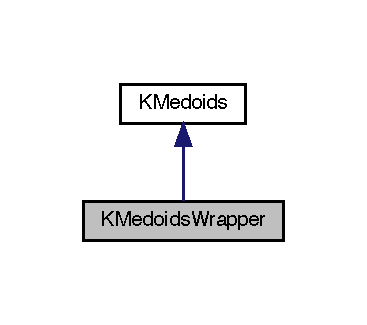
\includegraphics[width=176pt]{classKMedoidsWrapper__inherit__graph}
\end{center}
\end{figure}
\doxysubsection*{Public Member Functions}
\begin{DoxyCompactItemize}
\item 
void \mbox{\hyperlink{classKMedoidsWrapper_a3cffb0d5d82db7d6a8b9f62012ac169c}{fit\+Python}} (py\+::array\+\_\+t$<$ double $>$ input\+Data, std\+::string loss, int k, std\+::string \mbox{\hyperlink{classKMedoids_a3cf57e612442072fb377b1714fc5e12e}{log\+Filename}})
\begin{DoxyCompactList}\small\item\em Python binding for fitting a \mbox{\hyperlink{classKMedoids}{KMedoids}} object to the. \end{DoxyCompactList}\item 
py\+::array\+\_\+t$<$ double $>$ \mbox{\hyperlink{classKMedoidsWrapper_af24a4a55cc36ed02303e094c176427c3}{get\+Medoids\+Final\+Python}} ()
\begin{DoxyCompactList}\small\item\em Returns the final medoids. \end{DoxyCompactList}\item 
py\+::array\+\_\+t$<$ double $>$ \mbox{\hyperlink{classKMedoidsWrapper_a02d6751e6c126a4aa25909d37011853d}{get\+Medoids\+Build\+Python}} ()
\begin{DoxyCompactList}\small\item\em Returns the build medoids. \end{DoxyCompactList}\item 
py\+::array\+\_\+t$<$ double $>$ \mbox{\hyperlink{classKMedoidsWrapper_ae1da2fd6b272d0ddea14549cd18c2af8}{get\+Labels\+Python}} ()
\begin{DoxyCompactList}\small\item\em Returns the medoid assignments for each datapoint. \end{DoxyCompactList}\item 
int \mbox{\hyperlink{classKMedoidsWrapper_acfbcaf672bd1f1db1c00d35704341988}{get\+Steps\+Python}} ()
\begin{DoxyCompactList}\small\item\em Returns the number of swap steps. \end{DoxyCompactList}\item 
\mbox{\hyperlink{classKMedoidsWrapper_aa94dfc65454f847af5d08a2d7b816bb4}{KMedoids}} (int \mbox{\hyperlink{classKMedoids_a3365e728fd524c0be2fbab0b58e3a4cd}{n\+\_\+medoids}}=5, std\+::string \mbox{\hyperlink{classKMedoids_a849662ecdbd5164ab37f4bd4f3223344}{algorithm}}=\char`\"{}Bandit\+PAM\char`\"{}, int \mbox{\hyperlink{classKMedoids_a8d319c1a783be7c06205bf855b4976b5}{verbosity}}=0, int \mbox{\hyperlink{classKMedoids_a3f8f9d261e721749f14f30dacfe9aa03}{max\+\_\+iter}}=1000, std\+::string \mbox{\hyperlink{classKMedoids_a3cf57e612442072fb377b1714fc5e12e}{log\+Filename}}=\char`\"{}KMedoids\+Logfile\char`\"{})
\begin{DoxyCompactList}\small\item\em Class implementation for running \mbox{\hyperlink{classKMedoids}{KMedoids}} methods. \end{DoxyCompactList}\end{DoxyCompactItemize}


\doxysubsection{Detailed Description}
Python wrapper for \mbox{\hyperlink{classKMedoids}{KMedoids}} class. 

\mbox{\hyperlink{classKMedoidsWrapper}{KMedoids\+Wrapper}} class. Is the Python wrapper generated by Pybind that allows for calling the C++ code in Python. 

\doxysubsection{Member Function Documentation}
\mbox{\Hypertarget{classKMedoidsWrapper_a3cffb0d5d82db7d6a8b9f62012ac169c}\label{classKMedoidsWrapper_a3cffb0d5d82db7d6a8b9f62012ac169c}} 
\index{KMedoidsWrapper@{KMedoidsWrapper}!fitPython@{fitPython}}
\index{fitPython@{fitPython}!KMedoidsWrapper@{KMedoidsWrapper}}
\doxysubsubsection{\texorpdfstring{fitPython()}{fitPython()}}
{\footnotesize\ttfamily void KMedoids\+Wrapper\+::fit\+Python (\begin{DoxyParamCaption}\item[{py\+::array\+\_\+t$<$ double $>$}]{input\+Data,  }\item[{std\+::string}]{loss,  }\item[{int}]{k,  }\item[{std\+::string}]{log\+Filename }\end{DoxyParamCaption})\hspace{0.3cm}{\ttfamily [inline]}}



Python binding for fitting a \mbox{\hyperlink{classKMedoids}{KMedoids}} object to the. 

This is the primary function of the \mbox{\hyperlink{classKMedoids}{KMedoids}} module\+: this finds the build and swap medoids for the desired data


\begin{DoxyParams}{Parameters}
{\em input\+Data} & Input data to find the medoids of \\
\hline
{\em loss} & The loss function used during medoid computation \\
\hline
{\em k} & The number of medoids to compute \\
\hline
{\em log\+Filename} & The name of the outputted log file \\
\hline
\end{DoxyParams}
\mbox{\Hypertarget{classKMedoidsWrapper_ae1da2fd6b272d0ddea14549cd18c2af8}\label{classKMedoidsWrapper_ae1da2fd6b272d0ddea14549cd18c2af8}} 
\index{KMedoidsWrapper@{KMedoidsWrapper}!getLabelsPython@{getLabelsPython}}
\index{getLabelsPython@{getLabelsPython}!KMedoidsWrapper@{KMedoidsWrapper}}
\doxysubsubsection{\texorpdfstring{getLabelsPython()}{getLabelsPython()}}
{\footnotesize\ttfamily py\+::array\+\_\+t$<$double$>$ KMedoids\+Wrapper\+::get\+Labels\+Python (\begin{DoxyParamCaption}{ }\end{DoxyParamCaption})\hspace{0.3cm}{\ttfamily [inline]}}



Returns the medoid assignments for each datapoint. 

Returns as a numpy array the medoid each input datapoint is assigned to after \mbox{\hyperlink{classKMedoids_ae241800e72a6b4a677333ffbf06e1798}{KMedoids\+::fit}} is called and the final medoids have been identified \mbox{\Hypertarget{classKMedoidsWrapper_a02d6751e6c126a4aa25909d37011853d}\label{classKMedoidsWrapper_a02d6751e6c126a4aa25909d37011853d}} 
\index{KMedoidsWrapper@{KMedoidsWrapper}!getMedoidsBuildPython@{getMedoidsBuildPython}}
\index{getMedoidsBuildPython@{getMedoidsBuildPython}!KMedoidsWrapper@{KMedoidsWrapper}}
\doxysubsubsection{\texorpdfstring{getMedoidsBuildPython()}{getMedoidsBuildPython()}}
{\footnotesize\ttfamily py\+::array\+\_\+t$<$double$>$ KMedoids\+Wrapper\+::get\+Medoids\+Build\+Python (\begin{DoxyParamCaption}{ }\end{DoxyParamCaption})\hspace{0.3cm}{\ttfamily [inline]}}



Returns the build medoids. 

Returns as a numpy array the build medoids at the end of the BUILD step after \mbox{\hyperlink{classKMedoids_ae241800e72a6b4a677333ffbf06e1798}{KMedoids\+::fit}} has been called. \mbox{\Hypertarget{classKMedoidsWrapper_af24a4a55cc36ed02303e094c176427c3}\label{classKMedoidsWrapper_af24a4a55cc36ed02303e094c176427c3}} 
\index{KMedoidsWrapper@{KMedoidsWrapper}!getMedoidsFinalPython@{getMedoidsFinalPython}}
\index{getMedoidsFinalPython@{getMedoidsFinalPython}!KMedoidsWrapper@{KMedoidsWrapper}}
\doxysubsubsection{\texorpdfstring{getMedoidsFinalPython()}{getMedoidsFinalPython()}}
{\footnotesize\ttfamily py\+::array\+\_\+t$<$double$>$ KMedoids\+Wrapper\+::get\+Medoids\+Final\+Python (\begin{DoxyParamCaption}{ }\end{DoxyParamCaption})\hspace{0.3cm}{\ttfamily [inline]}}



Returns the final medoids. 

Returns as a numpy array the final medoids at the end of the SWAP step after \mbox{\hyperlink{classKMedoids_ae241800e72a6b4a677333ffbf06e1798}{KMedoids\+::fit}} has been called. \mbox{\Hypertarget{classKMedoidsWrapper_acfbcaf672bd1f1db1c00d35704341988}\label{classKMedoidsWrapper_acfbcaf672bd1f1db1c00d35704341988}} 
\index{KMedoidsWrapper@{KMedoidsWrapper}!getStepsPython@{getStepsPython}}
\index{getStepsPython@{getStepsPython}!KMedoidsWrapper@{KMedoidsWrapper}}
\doxysubsubsection{\texorpdfstring{getStepsPython()}{getStepsPython()}}
{\footnotesize\ttfamily int KMedoids\+Wrapper\+::get\+Steps\+Python (\begin{DoxyParamCaption}{ }\end{DoxyParamCaption})\hspace{0.3cm}{\ttfamily [inline]}}



Returns the number of swap steps. 

Returns the number of SWAP steps completed during the last call to \mbox{\hyperlink{classKMedoids_ae241800e72a6b4a677333ffbf06e1798}{KMedoids\+::fit}} \mbox{\Hypertarget{classKMedoidsWrapper_aa94dfc65454f847af5d08a2d7b816bb4}\label{classKMedoidsWrapper_aa94dfc65454f847af5d08a2d7b816bb4}} 
\index{KMedoidsWrapper@{KMedoidsWrapper}!KMedoids@{KMedoids}}
\index{KMedoids@{KMedoids}!KMedoidsWrapper@{KMedoidsWrapper}}
\doxysubsubsection{\texorpdfstring{KMedoids()}{KMedoids()}}
{\footnotesize\ttfamily KMedoids\+::\+KMedoids (\begin{DoxyParamCaption}\item[{int}]{n\+\_\+medoids = {\ttfamily 5},  }\item[{std\+::string}]{algorithm = {\ttfamily \char`\"{}BanditPAM\char`\"{}},  }\item[{int}]{verbosity = {\ttfamily 0},  }\item[{int}]{max\+\_\+iter = {\ttfamily 1000},  }\item[{std\+::string}]{log\+Filename = {\ttfamily \char`\"{}KMedoidsLogfile\char`\"{}} }\end{DoxyParamCaption})}



Class implementation for running \mbox{\hyperlink{classKMedoids}{KMedoids}} methods. 

\mbox{\hyperlink{classKMedoids}{KMedoids}} class. Creates a \mbox{\hyperlink{classKMedoids}{KMedoids}} object that can be used to find the medoids for a particular set of input data.


\begin{DoxyParams}{Parameters}
{\em n\+\_\+medoids} & Number of medoids/clusters to create \\
\hline
{\em algorithm} & Algorithm used to find medoids; options are \char`\"{}\+Bandit\+PAM\char`\"{} for the \char`\"{}\+Bandit-\/\+PAM\char`\"{} algorithm, or \char`\"{}naive\char`\"{} to use the naive method \\
\hline
{\em verbosity} & Verbosity of the algorithm, 0 will have no log file emitted, 1 will emit a log file \\
\hline
{\em max\+\_\+iter} & The maximum number of iterations the algorithm runs for \\
\hline
{\em log\+Filename} & The name of the output log file \\
\hline
\end{DoxyParams}


The documentation for this class was generated from the following file\+:\begin{DoxyCompactItemize}
\item 
/\+Users/dhavaldangaria/\+Bandit\+PAM/src/\mbox{\hyperlink{kmedoids__pywrapper_8cpp}{kmedoids\+\_\+pywrapper.\+cpp}}\end{DoxyCompactItemize}

\hypertarget{structLogHelper}{}\doxysection{Log\+Helper Struct Reference}
\label{structLogHelper}\index{LogHelper@{LogHelper}}


Logging class for structured \mbox{\hyperlink{classKMedoids}{KMedoids}} logs.  




{\ttfamily \#include $<$kmedoids\+\_\+ucb.\+hpp$>$}

\doxysubsection*{Public Member Functions}
\begin{DoxyCompactItemize}
\item 
void \mbox{\hyperlink{structLogHelper_a8bf957fb897ae5b548264f2f614879c5}{init}} (std\+::string input\+\_\+filename=\char`\"{}KMedoids\+Logfile\char`\"{})
\begin{DoxyCompactList}\small\item\em Opens the log file. \end{DoxyCompactList}\item 
void \mbox{\hyperlink{structLogHelper_a4624149f53c4577d0565f761c155d800}{close}} ()
\begin{DoxyCompactList}\small\item\em Closes the log file. \end{DoxyCompactList}\item 
void \mbox{\hyperlink{structLogHelper_a5b1a8ff2ae2ce6e3293e3b34085e3b86}{write\+Summary\+Line}} (std\+::string key, arma\+::rowvec vec)
\begin{DoxyCompactList}\small\item\em Writes a vector out for a given key. \end{DoxyCompactList}\item 
{\footnotesize template$<$typename T $>$ }\\void \mbox{\hyperlink{structLogHelper_ad1bb80fa2bd8b1dfcd944ea19c4e8e06}{write\+Log\+String\+Line}} (std\+::string key, std\+::vector$<$ T $>$ vec)
\begin{DoxyCompactList}\small\item\em Writes a logstring component. \end{DoxyCompactList}\item 
void \mbox{\hyperlink{structLogHelper_a15b3f49bf98956a0585f036801e25dbe}{write\+Profile}} (arma\+::rowvec b\+\_\+medoids, arma\+::rowvec f\+\_\+medoids, int steps, double loss)
\begin{DoxyCompactList}\small\item\em Writes formatted summary log of a \mbox{\hyperlink{classKMedoids}{KMedoids}} run. \end{DoxyCompactList}\end{DoxyCompactItemize}
\doxysubsection*{Public Attributes}
\begin{DoxyCompactItemize}
\item 
\mbox{\Hypertarget{structLogHelper_a084e11845451a653f46a48ab92c97ee8}\label{structLogHelper_a084e11845451a653f46a48ab92c97ee8}} 
std\+::ofstream {\bfseries hlog\+File}
\begin{DoxyCompactList}\small\item\em Output stream that writes the \mbox{\hyperlink{classKMedoids}{KMedoids}} log. \end{DoxyCompactList}\item 
\mbox{\Hypertarget{structLogHelper_a7f9490e07d6bfc71b0d0fd555ca4f530}\label{structLogHelper_a7f9490e07d6bfc71b0d0fd555ca4f530}} 
std\+::vector$<$ double $>$ {\bfseries comp\+\_\+exact\+\_\+build}
\begin{DoxyCompactList}\small\item\em Number of computations in build step. \end{DoxyCompactList}\item 
\mbox{\Hypertarget{structLogHelper_aaee1d830760c6b497f2fad31a0e368f8}\label{structLogHelper_aaee1d830760c6b497f2fad31a0e368f8}} 
std\+::vector$<$ double $>$ {\bfseries comp\+\_\+exact\+\_\+swap}
\begin{DoxyCompactList}\small\item\em Number of computations in swap step. \end{DoxyCompactList}\item 
\mbox{\Hypertarget{structLogHelper_a8da7e85d166977478fcfe848bb739dfa}\label{structLogHelper_a8da7e85d166977478fcfe848bb739dfa}} 
std\+::vector$<$ double $>$ {\bfseries loss\+\_\+build}
\begin{DoxyCompactList}\small\item\em Loss after each iteration of build step. \end{DoxyCompactList}\item 
\mbox{\Hypertarget{structLogHelper_a3361ae9284a7fca5b867165e0380af4b}\label{structLogHelper_a3361ae9284a7fca5b867165e0380af4b}} 
std\+::vector$<$ double $>$ {\bfseries loss\+\_\+swap}
\begin{DoxyCompactList}\small\item\em Loss after each iteration of swap step. \end{DoxyCompactList}\item 
\mbox{\Hypertarget{structLogHelper_aed75dac28380b3f67b777d6b36719aa9}\label{structLogHelper_aed75dac28380b3f67b777d6b36719aa9}} 
std\+::vector$<$ double $>$ {\bfseries p\+\_\+build}
\begin{DoxyCompactList}\small\item\em Precision for each iteration of build step. \end{DoxyCompactList}\item 
\mbox{\Hypertarget{structLogHelper_a87a35e651ad2a32092777e1d9bd4acfa}\label{structLogHelper_a87a35e651ad2a32092777e1d9bd4acfa}} 
std\+::vector$<$ double $>$ {\bfseries p\+\_\+swap}
\begin{DoxyCompactList}\small\item\em Precision for each iteration of swap step. \end{DoxyCompactList}\item 
\mbox{\Hypertarget{structLogHelper_a835a54928567970dd564d9eaed87597c}\label{structLogHelper_a835a54928567970dd564d9eaed87597c}} 
std\+::vector$<$ std\+::string $>$ {\bfseries sigma\+\_\+build}
\begin{DoxyCompactList}\small\item\em Distributions for each iteration of build step. \end{DoxyCompactList}\item 
\mbox{\Hypertarget{structLogHelper_afee211952d9a61c217622557e91c1275}\label{structLogHelper_afee211952d9a61c217622557e91c1275}} 
std\+::vector$<$ std\+::string $>$ {\bfseries sigma\+\_\+swap}
\begin{DoxyCompactList}\small\item\em Distributions for each iteration of swap step. \end{DoxyCompactList}\end{DoxyCompactItemize}


\doxysubsection{Detailed Description}
Logging class for structured \mbox{\hyperlink{classKMedoids}{KMedoids}} logs. 

\mbox{\hyperlink{structLogHelper}{Log\+Helper}} class. Assists the \mbox{\hyperlink{classKMedoids}{KMedoids}} class in structured logging. 

\doxysubsection{Member Function Documentation}
\mbox{\Hypertarget{structLogHelper_a4624149f53c4577d0565f761c155d800}\label{structLogHelper_a4624149f53c4577d0565f761c155d800}} 
\index{LogHelper@{LogHelper}!close@{close}}
\index{close@{close}!LogHelper@{LogHelper}}
\doxysubsubsection{\texorpdfstring{close()}{close()}}
{\footnotesize\ttfamily void Log\+Helper\+::close (\begin{DoxyParamCaption}{ }\end{DoxyParamCaption})\hspace{0.3cm}{\ttfamily [inline]}}



Closes the log file. 

Closes the log file. \mbox{\Hypertarget{structLogHelper_a8bf957fb897ae5b548264f2f614879c5}\label{structLogHelper_a8bf957fb897ae5b548264f2f614879c5}} 
\index{LogHelper@{LogHelper}!init@{init}}
\index{init@{init}!LogHelper@{LogHelper}}
\doxysubsubsection{\texorpdfstring{init()}{init()}}
{\footnotesize\ttfamily void Log\+Helper\+::init (\begin{DoxyParamCaption}\item[{std\+::string}]{input\+\_\+filename = {\ttfamily \char`\"{}KMedoidsLogfile\char`\"{}} }\end{DoxyParamCaption})\hspace{0.3cm}{\ttfamily [inline]}}



Opens the log file. 

Opens the log file.


\begin{DoxyParams}{Parameters}
{\em input\+\_\+filename} & Filename that log will be saved as. \\
\hline
\end{DoxyParams}
\mbox{\Hypertarget{structLogHelper_ad1bb80fa2bd8b1dfcd944ea19c4e8e06}\label{structLogHelper_ad1bb80fa2bd8b1dfcd944ea19c4e8e06}} 
\index{LogHelper@{LogHelper}!writeLogStringLine@{writeLogStringLine}}
\index{writeLogStringLine@{writeLogStringLine}!LogHelper@{LogHelper}}
\doxysubsubsection{\texorpdfstring{writeLogStringLine()}{writeLogStringLine()}}
{\footnotesize\ttfamily template$<$typename T $>$ \\
void Log\+Helper\+::write\+Log\+String\+Line (\begin{DoxyParamCaption}\item[{std\+::string}]{key,  }\item[{std\+::vector$<$ T $>$}]{vec }\end{DoxyParamCaption})\hspace{0.3cm}{\ttfamily [inline]}}



Writes a logstring component. 

Writes a logstring line for the write\+Profile function.


\begin{DoxyParams}{Parameters}
{\em key} & Key for json-\/ified output structure \\
\hline
{\em vec} & Vector to be iterated across when writing logstring line \\
\hline
\end{DoxyParams}
\mbox{\Hypertarget{structLogHelper_a15b3f49bf98956a0585f036801e25dbe}\label{structLogHelper_a15b3f49bf98956a0585f036801e25dbe}} 
\index{LogHelper@{LogHelper}!writeProfile@{writeProfile}}
\index{writeProfile@{writeProfile}!LogHelper@{LogHelper}}
\doxysubsubsection{\texorpdfstring{writeProfile()}{writeProfile()}}
{\footnotesize\ttfamily void Log\+Helper\+::write\+Profile (\begin{DoxyParamCaption}\item[{arma\+::rowvec}]{b\+\_\+medoids,  }\item[{arma\+::rowvec}]{f\+\_\+medoids,  }\item[{int}]{steps,  }\item[{double}]{loss }\end{DoxyParamCaption})\hspace{0.3cm}{\ttfamily [inline]}}



Writes formatted summary log of a \mbox{\hyperlink{classKMedoids}{KMedoids}} run. 

Writes summary statistics of a \mbox{\hyperlink{classKMedoids}{KMedoids}} run. Statistics include medoids after the build step, medoids after the swap step, number of swap steps, the final loss, and logstrings of the number of points that had distance computations, loss, precision, and uncertainty for each iteration of both the build and swap steps.


\begin{DoxyParams}{Parameters}
{\em b\+\_\+medoids} & Medoids after the build step. \\
\hline
{\em f\+\_\+medoids} & Medoids after the swap step (final medoids). \\
\hline
{\em steps} & Number of swap steps. \\
\hline
{\em loss} & Final loss of the \mbox{\hyperlink{classKMedoids}{KMedoids}} object. \\
\hline
\end{DoxyParams}
\mbox{\Hypertarget{structLogHelper_a5b1a8ff2ae2ce6e3293e3b34085e3b86}\label{structLogHelper_a5b1a8ff2ae2ce6e3293e3b34085e3b86}} 
\index{LogHelper@{LogHelper}!writeSummaryLine@{writeSummaryLine}}
\index{writeSummaryLine@{writeSummaryLine}!LogHelper@{LogHelper}}
\doxysubsubsection{\texorpdfstring{writeSummaryLine()}{writeSummaryLine()}}
{\footnotesize\ttfamily void Log\+Helper\+::write\+Summary\+Line (\begin{DoxyParamCaption}\item[{std\+::string}]{key,  }\item[{arma\+::rowvec}]{vec }\end{DoxyParamCaption})\hspace{0.3cm}{\ttfamily [inline]}}



Writes a vector out for a given key. 

Writes a vector out for a given key


\begin{DoxyParams}{Parameters}
{\em key} & Key for json-\/ified output structure \\
\hline
{\em vec} & Vector to be iterated across when writing line \\
\hline
\end{DoxyParams}


The documentation for this struct was generated from the following file\+:\begin{DoxyCompactItemize}
\item 
/\+Users/dhavaldangaria/\+Bandit\+PAM/headers/kmedoids\+\_\+ucb.\+hpp\end{DoxyCompactItemize}

\chapter{File Documentation}
\hypertarget{kmedoids__ucb_8cpp}{}\doxysection{/\+Users/dhavaldangaria/\+Bandit\+PAM/src/kmedoids\+\_\+ucb.cpp File Reference}
\label{kmedoids__ucb_8cpp}\index{/Users/dhavaldangaria/BanditPAM/src/kmedoids\_ucb.cpp@{/Users/dhavaldangaria/BanditPAM/src/kmedoids\_ucb.cpp}}
{\ttfamily \#include \char`\"{}kmedoids\+\_\+ucb.\+hpp\char`\"{}}\newline
{\ttfamily \#include $<$armadillo$>$}\newline
{\ttfamily \#include $<$unordered\+\_\+map$>$}\newline
{\ttfamily \#include $<$regex$>$}\newline
Include dependency graph for kmedoids\+\_\+ucb.\+cpp\+:
\nopagebreak
\begin{figure}[H]
\begin{center}
\leavevmode
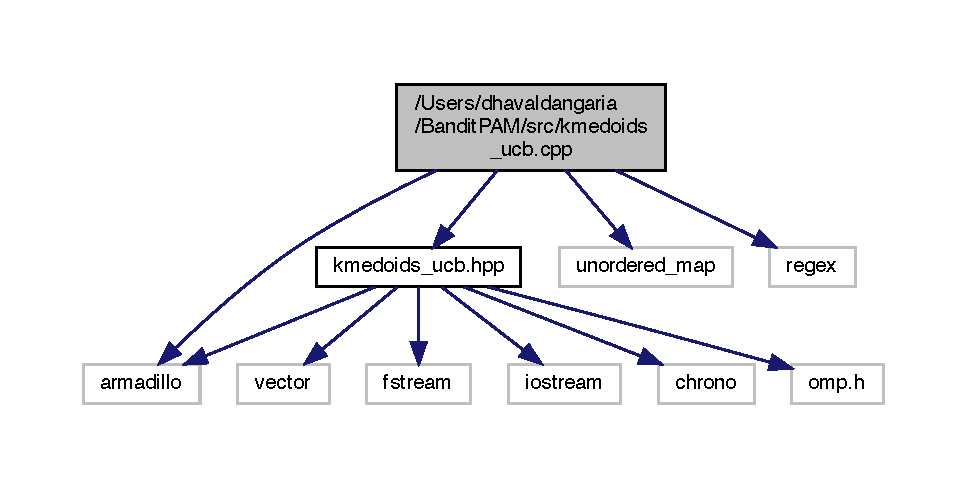
\includegraphics[width=350pt]{kmedoids__ucb_8cpp__incl}
\end{center}
\end{figure}


\doxysubsection{Detailed Description}
\begin{DoxyDate}{Date}
2020-\/06-\/10
\end{DoxyDate}
This file contains the primary C++ implementation of the Bandit\+PAM code. 

\hypertarget{kmedoids__pywrapper_8cpp}{}\doxysection{/\+Users/dhavaldangaria/\+Bandit\+PAM/src/kmedoids\+\_\+pywrapper.cpp File Reference}
\label{kmedoids__pywrapper_8cpp}\index{/Users/dhavaldangaria/BanditPAM/src/kmedoids\_pywrapper.cpp@{/Users/dhavaldangaria/BanditPAM/src/kmedoids\_pywrapper.cpp}}
{\ttfamily \#include \char`\"{}kmedoids\+\_\+ucb.\+hpp\char`\"{}}\newline
{\ttfamily \#include $<$armadillo$>$}\newline
{\ttfamily \#include $<$carma$>$}\newline
{\ttfamily \#include $<$pybind11/pybind11.\+h$>$}\newline
{\ttfamily \#include $<$pybind11/numpy.\+h$>$}\newline
Include dependency graph for kmedoids\+\_\+pywrapper.\+cpp\+:
\nopagebreak
\begin{figure}[H]
\begin{center}
\leavevmode
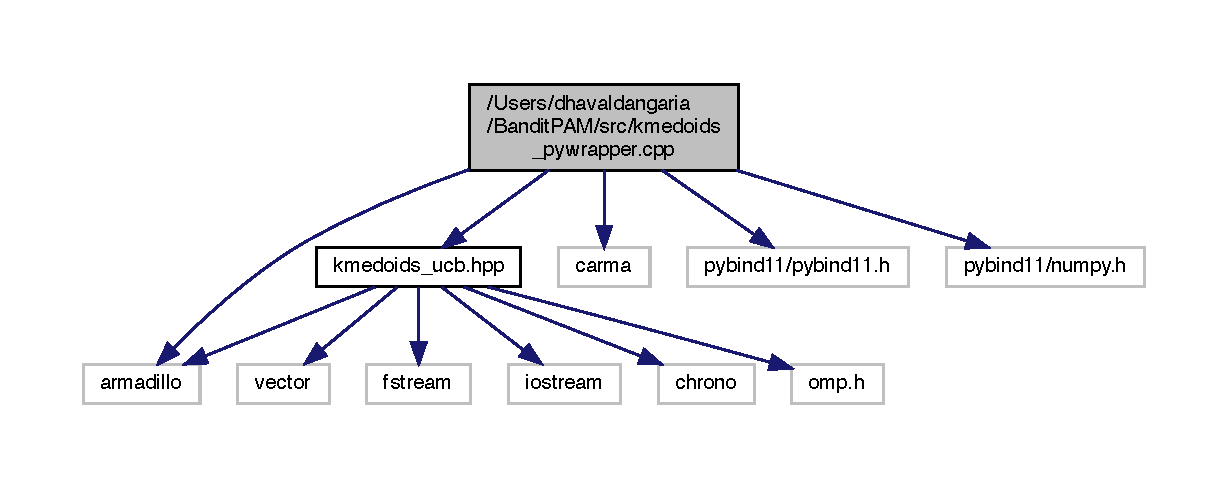
\includegraphics[width=350pt]{kmedoids__pywrapper_8cpp__incl}
\end{center}
\end{figure}
\doxysubsection*{Classes}
\begin{DoxyCompactItemize}
\item 
class \mbox{\hyperlink{classKMedoidsWrapper}{KMedoids\+Wrapper}}
\begin{DoxyCompactList}\small\item\em Python wrapper for \mbox{\hyperlink{classKMedoids}{KMedoids}} class. \end{DoxyCompactList}\end{DoxyCompactItemize}
\doxysubsection*{Functions}
\begin{DoxyCompactItemize}
\item 
\mbox{\Hypertarget{kmedoids__pywrapper_8cpp_a66c5e3323d71e29a0a148bec731ac27b}\label{kmedoids__pywrapper_8cpp_a66c5e3323d71e29a0a148bec731ac27b}} 
{\bfseries PYBIND11\+\_\+\+MODULE} (Bandit\+PAM, m)
\end{DoxyCompactItemize}


\doxysubsection{Detailed Description}
\begin{DoxyDate}{Date}
2020-\/06-\/10
\end{DoxyDate}
Creates the Python bindings for the C++ code that allows it to be called in Python. 

\hypertarget{main_8cpp}{}\doxysection{/\+Users/dhavaldangaria/\+Bandit\+PAM/src/main.cpp File Reference}
\label{main_8cpp}\index{/Users/dhavaldangaria/BanditPAM/src/main.cpp@{/Users/dhavaldangaria/BanditPAM/src/main.cpp}}
{\ttfamily \#include \char`\"{}kmedoids\+\_\+ucb.\+hpp\char`\"{}}\newline
{\ttfamily \#include $<$armadillo$>$}\newline
{\ttfamily \#include $<$chrono$>$}\newline
{\ttfamily \#include $<$fstream$>$}\newline
{\ttfamily \#include $<$unistd.\+h$>$}\newline
{\ttfamily \#include $<$exception$>$}\newline
{\ttfamily \#include $<$regex$>$}\newline
Include dependency graph for main.\+cpp\+:
\nopagebreak
\begin{figure}[H]
\begin{center}
\leavevmode
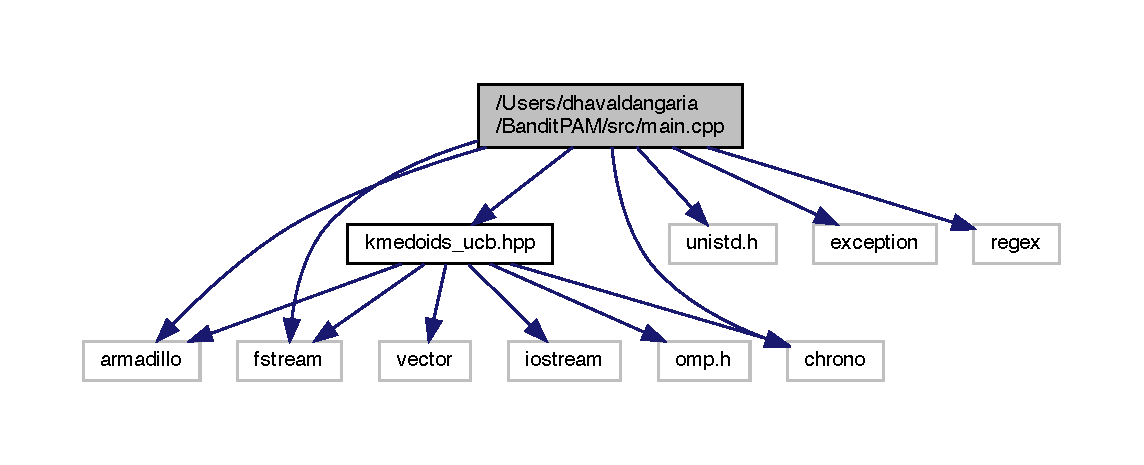
\includegraphics[width=350pt]{main_8cpp__incl}
\end{center}
\end{figure}
\doxysubsection*{Functions}
\begin{DoxyCompactItemize}
\item 
\mbox{\Hypertarget{main_8cpp_a0ddf1224851353fc92bfbff6f499fa97}\label{main_8cpp_a0ddf1224851353fc92bfbff6f499fa97}} 
int {\bfseries main} (int argc, char $\ast$argv\mbox{[}$\,$\mbox{]})
\end{DoxyCompactItemize}


\doxysubsection{Detailed Description}
\begin{DoxyDate}{Date}
2020-\/06-\/10
\end{DoxyDate}
Defines a command line program that can be used to run the Bandit\+PAM \mbox{\hyperlink{classKMedoids}{KMedoids}} algorithm.

Usage (from home repo directory)\+: ./src/build/\+Bandit\+PAM -\/f \mbox{[}path/to/input\mbox{]} -\/k \mbox{[}number of clusters\mbox{]} 

%--- End generated contents ---

% Index
\backmatter
\newpage
\phantomsection
\clearemptydoublepage
\addcontentsline{toc}{chapter}{Index}
\printindex

\end{document}
